\documentclass[11pt]{article}
\usepackage[a4paper,margin=25mm,marginparwidth=20mm]{geometry}
\usepackage{fontspec}
\usepackage{amsmath,amssymb,mathtools}
\usepackage{unicode-math}
\usepackage[normalem]{ulem}
\usepackage{graphicx,xcolor,tikz,tikz-cd}
\usetikzlibrary{calc,decorations.pathmorphing,decorations.pathreplacing,arrows.meta,shapes.geometric}
\newcommand{\scanpage}[1]{\par\medskip\noindent{\footnotesize\textcolor{gray}{[scan #1]}}\par}
\newcommand{\mspage}[1]{{\footnotesize\textcolor{gray}{[p.~#1]}}\ }
\newcommand{\unsure}[1]{{\color{blue}#1}}
\newcommand{\illegible}[1]{\textcolor{red}{[illeg.~#1]}}
\newcommand{\deleted}[1]{{\color{gray}#1}}
\newcommand{\inserted}[1]{{\color{teal}#1}}
\newcommand{\margin}[1]{\ifinner{\footnotesize[#1]}\else\marginpar{\footnotesize #1}\fi}
\newcommand{\diagram}[1]{\ifmmode\vcenter{\hbox{#1}}\else\ifinner #1\else\par\begin{center}#1\end{center}\par\fi\fi}
\let\figure\relax\newcommand{\figure}[1]{\ifmmode\vcenter{\hbox{#1}}\else\ifinner #1\else\par\begin{center}#1\end{center}\par\fi\fi}
\raggedbottom
\usepackage{newunicodechar}
\newfontfamily\cyrfont{DejaVu Serif}[Scale=MatchLowercase]
\newunicodechar{А}{{\cyrfont\char"0410}}
\newunicodechar{Б}{{\cyrfont\char"0411}}
\newunicodechar{В}{{\cyrfont\char"0412}}
\newunicodechar{Г}{{\cyrfont\char"0413}}
\newunicodechar{Д}{{\cyrfont\char"0414}}
\newunicodechar{Е}{{\cyrfont\char"0415}}
\newunicodechar{Ж}{{\cyrfont\char"0416}}
\newunicodechar{З}{{\cyrfont\char"0417}}
\newunicodechar{И}{{\cyrfont\char"0418}}
\newunicodechar{Й}{{\cyrfont\char"0419}}
\newunicodechar{К}{{\cyrfont\char"041A}}
\newunicodechar{Л}{{\cyrfont\char"041B}}
\newunicodechar{М}{{\cyrfont\char"041C}}
\newunicodechar{Н}{{\cyrfont\char"041D}}
\newunicodechar{О}{{\cyrfont\char"041E}}
\newunicodechar{П}{{\cyrfont\char"041F}}
\newunicodechar{Р}{{\cyrfont\char"0420}}
\newunicodechar{С}{{\cyrfont\char"0421}}
\newunicodechar{Т}{{\cyrfont\char"0422}}
\newunicodechar{У}{{\cyrfont\char"0423}}
\newunicodechar{Ф}{{\cyrfont\char"0424}}
\newunicodechar{Х}{{\cyrfont\char"0425}}
\newunicodechar{Ц}{{\cyrfont\char"0426}}
\newunicodechar{Ч}{{\cyrfont\char"0427}}
\newunicodechar{Ш}{{\cyrfont\char"0428}}
\newunicodechar{Щ}{{\cyrfont\char"0429}}
\newunicodechar{Ъ}{{\cyrfont\char"042A}}
\newunicodechar{Ы}{{\cyrfont\char"042B}}
\newunicodechar{Ь}{{\cyrfont\char"042C}}
\newunicodechar{Э}{{\cyrfont\char"042D}}
\newunicodechar{Ю}{{\cyrfont\char"042E}}
\newunicodechar{Я}{{\cyrfont\char"042F}}
\newunicodechar{а}{{\cyrfont\char"0430}}
\newunicodechar{б}{{\cyrfont\char"0431}}
\newunicodechar{в}{{\cyrfont\char"0432}}
\newunicodechar{г}{{\cyrfont\char"0433}}
\newunicodechar{д}{{\cyrfont\char"0434}}
\newunicodechar{е}{{\cyrfont\char"0435}}
\newunicodechar{ж}{{\cyrfont\char"0436}}
\newunicodechar{з}{{\cyrfont\char"0437}}
\newunicodechar{и}{{\cyrfont\char"0438}}
\newunicodechar{й}{{\cyrfont\char"0439}}
\newunicodechar{к}{{\cyrfont\char"043A}}
\newunicodechar{л}{{\cyrfont\char"043B}}
\newunicodechar{м}{{\cyrfont\char"043C}}
\newunicodechar{н}{{\cyrfont\char"043D}}
\newunicodechar{о}{{\cyrfont\char"043E}}
\newunicodechar{п}{{\cyrfont\char"043F}}
\newunicodechar{р}{{\cyrfont\char"0440}}
\newunicodechar{с}{{\cyrfont\char"0441}}
\newunicodechar{т}{{\cyrfont\char"0442}}
\newunicodechar{у}{{\cyrfont\char"0443}}
\newunicodechar{ф}{{\cyrfont\char"0444}}
\newunicodechar{х}{{\cyrfont\char"0445}}
\newunicodechar{ц}{{\cyrfont\char"0446}}
\newunicodechar{ч}{{\cyrfont\char"0447}}
\newunicodechar{ш}{{\cyrfont\char"0448}}
\newunicodechar{щ}{{\cyrfont\char"0449}}
\newunicodechar{ъ}{{\cyrfont\char"044A}}
\newunicodechar{ы}{{\cyrfont\char"044B}}
\newunicodechar{ь}{{\cyrfont\char"044C}}
\newunicodechar{э}{{\cyrfont\char"044D}}
\newunicodechar{ю}{{\cyrfont\char"044E}}
\newunicodechar{я}{{\cyrfont\char"044F}}
\newunicodechar{≃}{\ensuremath{\simeq}}
\setmathfont{Latin Modern Math}
\setmathfont{STIX Two Math}[range={"27CB,"27CD}]

% ---- typesetting pass of the readers (reader_typeset.py, 13 Nov 2026): fit to the page; links to the scans ----
\usepackage{luacode}
\newattribute\LMattr
\newcount\LMscanvalue
\tolerance=1000 \emergencystretch=3em \tracinglostchars=3
\begin{luacode*}
LMFIT = LMFIT or {}
local F = LMFIT
F.measure = false   -- a trial setting of a marginal note: record the widths, change nothing
F.maxw = 0          -- widest natural line of the trial (sp)
F.inpar = false
F.A = luatexbase.registernumber("LMattr")
F.n = {scaled_display = 0, rotated_display = 0, scaled_line = 0, rotated_line = 0, small_line = 0}
local HLIST, GLUE, KERN, WHATSIT, GLYPH = node.id("hlist"), node.id("glue"), node.id("kern"), node.id("whatsit"), node.id("glyph")
local SETMATRIX = node.subtype("pdf_setmatrix")
local MINSCALE = 0.70
local function note(kind, s, extra)
  F.n[kind] = (F.n[kind] or 0) + 1
  texio.write_nl("log", string.format("LMFIT %s scale %.3f at input line %d%s", kind, s, tex.inputlineno, extra or ""))
end
local function matrix(a, b, c, d)
  local n = node.new(WHATSIT, SETMATRIX)
  n.data = string.format("%.8f %.8f %.8f %.8f", a, b, c, d)
  return n
end
local function kern(w)
  local k = node.new(KERN, 1)
  k.kern = w
  return k
end
local function chain(...)
  local t = {...}
  for i = 1, #t do
    t[i].prev = t[i - 1]
    t[i].next = t[i + 1]
  end
  return t[1]
end
-- b: a box at its natural width. Returns a list that draws b scaled by s (about its reference point) and takes up
-- the scaled width; the matrix is undone at the same point, so colours that run on after the box are kept.
local function scaled(b, s)
  return chain(matrix(s, 0, 0, s), b, kern(-b.width), matrix(1 / s, 0, 0, 1 / s), kern(math.floor(s * b.width)))
end
-- b turned 90 degrees counter-clockwise and scaled by s: width s(h+d), height s*w
local function rotated(b, s, left)
  return chain(kern(left + math.floor(s * b.height)), matrix(0, s, -s, 0), b, kern(-b.width), matrix(0, -1 / s, 1 / s, 0),
               kern(math.floor(s * b.depth)))
end
local function rotscale(w)
  local room = 0.92 * tex.vsize
  if room < 100 * 65536 then room = 600 * 65536 end
  return math.min(1, room / w)
end

local function fit_lines(head)
  F.inpar = false
  for line in node.traverse_id(HLIST, head) do
    if line.subtype == 1 and line.head and line.width > 10 * 65536 then
      local nw = node.dimensions(line.head)
      if F.measure and nw > F.maxw then F.maxw = nw end
      if nw > line.width + 6554 then
        local shrink, inf, glyphs = 0, false, false
        for n in node.traverse(line.head) do
          if n.id == GLUE then
            if n.shrink_order > 0 and n.shrink ~= 0 then inf = true else shrink = shrink + n.shrink end
          elseif n.id == GLYPH then
            glyphs = true
          end
        end
        if not inf and nw - shrink > line.width + 6554 and not F.measure then
          local s = line.width / nw
          local b = node.hpack(line.head)
          node.unset_attribute(b, LMFIT.A)
          if s >= MINSCALE or glyphs then
            line.head = scaled(b, s)
            if s >= MINSCALE then note("scaled_line", s) else note("small_line", s) end
          else
            local r = rotscale(nw)
            local w2 = r * (b.height + b.depth)
            line.head = rotated(b, r, math.max(0, math.floor((line.width - w2) / 2)))
            line.height = math.floor(r * nw)
            line.depth = 0
            note("rotated_line", r)
          end
          line.glue_set, line.glue_sign, line.glue_order = 0, 0, 0
        end
      end
    end
  end
  return head
end

local prev = {}
local function fit_display(head, display_type, need_penalties)
  if not head then return head end
  if display_type ~= "display" then
    prev.text = true
    prev.w = node.dimensions(head)
    return head
  end
  local z = tex.displaywidth
  local w = node.dimensions(head)
  local q = 0
  local tag = token.get_macro("df@tag")
  if tag and tag ~= "" and prev.text then q = prev.w + tex.getmath("quad", "text") end
  prev.text = false
  if F.measure then
    if w + q > F.maxw then F.maxw = w + q end
    return head
  end
  if z < 10 * 65536 or w <= z - q + 6554 then return head end
  local shrink = 0
  for n in node.traverse_id(GLUE, head) do
    if n.shrink_order > 0 and n.shrink ~= 0 then return head end
    shrink = shrink + n.shrink
  end
  if w - shrink <= z - q then return head end
  local target = z - q
  if target / w < MINSCALE then target = z end   -- the tag goes on a line of its own
  local s = target / w
  local b = node.hpack(head)
  node.unset_attribute(b, LMFIT.A)
  local h, d = b.height, b.depth
  local nb
  if s >= MINSCALE then
    nb = node.hpack(scaled(b, s))
    nb.width, nb.height, nb.depth = math.floor(target) - 2, math.floor(s * h) + 1, math.floor(s * d) + 1
    note("scaled_display", s)
  else
    local r = rotscale(w)
    nb = node.hpack(rotated(b, r, 0))
    nb.width, nb.height, nb.depth = math.floor(r * (h + d)) + 1, math.floor(r * w) + 1, 0
    note("rotated_display", r)
  end
  return nb
end

luatexbase.add_to_callback("pre_linebreak_filter", function(head) F.inpar = true return head end, "lmfit.pre")
luatexbase.add_to_callback("post_linebreak_filter", fit_lines, "lmfit.lines")
luatexbase.add_to_callback("hpack_filter", function(head) F.inpar = false return head end, "lmfit.hpack")
luatexbase.add_to_callback("post_mlist_to_hlist_filter", fit_display, "lmfit.display")
-- TeX reports an overfull line while it breaks the paragraph, before the line is repaired above: such reports are
-- dropped; every other overfull box is reported in TeX's words.
luatexbase.add_to_callback("hpack_quality", function(incident, detail, head, first, last)
  if incident == "overfull" and not F.inpar and not F.measure then
    texio.write_nl("log", string.format("Overfull \\hbox (%.5fpt too wide) not repaired, at lines %d--%d", detail / 65536, first, last))
  end
end, "lmfit.quality")

-- Links to the scans. \unsure and \illegible set the attribute LMattr to (number of the cote) * 10000 + scan; when a
-- page is shipped out, every run of marked material inside one line or box becomes one link annotation. (A link made
-- with \href cannot hold a paragraph break and must start and end in the same box; these marks do neither.)
local A = luatexbase.registernumber("LMattr")
local VLIST, PENALTY, MATH = node.id("vlist"), node.id("penalty"), node.id("math")
local STARTLINK, ENDLINK, ACTION = node.subtype("pdf_start_link"), node.subtype("pdf_end_link"), node.subtype("pdf_action")
local inert = {[GLUE] = true, [KERN] = true, [PENALTY] = true, [WHATSIT] = true, [MATH] = true}
F.cotes = {}
F.links = 0
function F.at(cote, scan)
  local n = string.match(scan, "^%s*(%d+)")
  if cote == "" or not n then return end
  local k
  for i, c in ipairs(F.cotes) do if c == cote then k = i end end
  if not k then F.cotes[#F.cotes + 1] = cote k = #F.cotes end
  tex.setcount("global", "LMscanvalue", k * 10000 + tonumber(n))
end
local function url(v)
  return "https://grothendieck.umontpellier.fr/web/viewer.html?file=../" .. F.cotes[v // 10000] .. ".pdf#page=" .. (v % 10000)
end
local link_lists
local function link_runs(box)
  local n = box.head
  while n do
    local v = node.has_attribute(n, A)
    if v and v > 0 and not inert[n.id] then
      local last, m = n, n.next
      while m do
        if inert[m.id] then
        elseif node.has_attribute(m, A) == v then last = m
        else break end
        m = m.next
      end
      local w, h, d = node.dimensions(box.glue_set, box.glue_sign, box.glue_order, n, last.next)
      local s = node.new(WHATSIT, STARTLINK)
      s.width, s.height, s.depth = w, h, d
      local a = node.new(WHATSIT, ACTION)
      a.action_type = 3
      a.data = "/Subtype/Link/Border[0 0 0]/A<</Type/Action/S/URI/URI(" .. url(v) .. ")>>"
      s.action = a
      local e = node.new(WHATSIT, ENDLINK)
      box.head = node.insert_before(box.head, n, s)
      node.insert_after(box.head, last, e)
      F.links = F.links + 1
      n = e.next
    else
      if n.id == HLIST then link_runs(n) elseif n.id == VLIST then link_lists(n) end
      n = n.next
    end
  end
end
link_lists = function(box)
  for n in node.traverse(box.head) do
    if n.id == HLIST then link_runs(n) elseif n.id == VLIST then link_lists(n) end
  end
end
luatexbase.add_to_callback("pre_shipout_filter", function(box)
  if box.id == HLIST then link_runs(box) elseif box.id == VLIST then link_lists(box) end
  return true
end, "lmfit.links")
function F.summary()
  for k, v in pairs(F.n) do texio.write_nl("log", "LMFIT-SUMMARY " .. k .. " " .. v) end
  texio.write_nl("log", "LMFIT-SUMMARY links " .. F.links)
end
\end{luacode*}
\makeatletter
\AtEndDocument{\directlua{LMFIT.summary()}}
% a \simeq or \Gamma that stands outside a formula (a diagram label set as text) is set as mathematics: the text font
% has neither sign
\AtBeginDocument{\let\LMsimeq\simeq \protected\def\simeq{\ifmmode\LMsimeq\else$\LMsimeq$\fi}%
  \let\LMGamma\Gamma \protected\def\Gamma{\ifmmode\LMGamma\else$\LMGamma$\fi}}
% the page number and the placing of marginal notes are not part of a marked passage that runs over a page break
\output\expandafter{\expandafter\unsetattribute\expandafter\LMattr\the\output}
% -- links to the scans
\gdef\LMcotename{}
\newcommand\LMcote[1]{\gdef\LMcotename{#1}}
\newcommand\LMmark{\ifnum\LMscanvalue>0 \LMattr=\LMscanvalue\relax\fi}
\renewcommand{\scanpage}[1]{\directlua{LMFIT.at("\luaescapestring{\LMcotename}", "\luaescapestring{\detokenize{#1}}")}%
  \par\medskip\noindent{\footnotesize\LMmark\textcolor{gray}{[scan #1]}}\par}
\renewcommand{\unsure}[1]{{\color{blue}\LMmark #1}}
\renewcommand{\illegible}[1]{{\LMmark\textcolor{red}{[illeg.~#1]}}}
% -- marginal notes
\newsavebox\LMmbox
\newdimen\LMmw
\newdimen\LMmh
\newcommand\LMmarginstyle{\footnotesize\rightskip=0pt plus 2.5em\relax\parfillskip=0pt plus 1fil\relax\hyphenpenalty=50\relax
  \def\margin##1{{[##1]}}}
\newcommand\LMtrial[2]{% #1 a width, #2 the note: \LMmw its widest natural line, \LMmh its height
  \directlua{LMFIT.measure = true LMFIT.maxw = 0}%
  \setbox\LMmbox\vbox{\hsize=#1\relax\@parboxrestore\LMmarginstyle #2\par}%
  \directlua{LMFIT.measure = false tex.setdimen("LMmw", LMFIT.maxw)}%
  \LMmh=\dimexpr\ht\LMmbox+\dp\LMmbox\relax}
\newcommand\LMblock{\nobreak\vskip 3pt\moveright\@totalleftmargin\hbox to\linewidth{\hfill
  {\color{gray}\vrule width .6pt}\hskip 5pt\box\LMmbox}\vskip 3pt}
\newcommand\LMinblock[1]{%
  \LMtrial{.62\linewidth}{#1}%
  \ifdim\LMmw>.62\linewidth
    \ifdim\LMmw>\dimexpr\linewidth-6pt\relax \LMmw=\dimexpr\linewidth-6pt\relax \fi
  \else \advance\LMmw 0.5pt \fi
  \setbox\LMmbox\vbox{\hsize=\LMmw\@parboxrestore\LMmarginstyle #1\par}%
  \ifhmode \@bsphack\vadjust{\LMblock}\@esphack \else \LMblock \fi}
\newcommand\LMmargin[1]{\begingroup
  \LMtrial{\marginparwidth}{\rightskip=5pt plus 2.5em\relax #1}%
  \ifdim\LMmw>1.18\marginparwidth \LMinblock{#1}%
  \else\ifdim\LMmh>35pt \LMinblock{#1}%
  \else \marginpar{\LMmarginstyle\rightskip=5pt plus 2.5em\relax #1}%
  \fi\fi
  \endgroup}
\renewcommand{\margin}[1]{\ifinner{\footnotesize[#1]}\else\ifmmode{\footnotesize[#1]}\else\LMmargin{#1}\fi\fi}
\makeatother
% ---- end of the typesetting pass ----
\begin{document}
\LMcote{140-1}
\section*{La Longue Marche, cote 140-1 (draft)}

{\small\noindent Transcription diplomatique du manuscrit, faite par IA. Les lectures incertaines sont en
{\color{blue}bleu} (deux lectures possibles sont séparées par une barre, A|B), \textcolor{red}{[illeg.~$n$]} tient lieu
de $n$ mots illisibles, les mots biffés sont en {\color{gray}gris}, les ajouts entre les lignes en {\color{teal}bleu-vert}.
Chaque lecture en bleu, chaque \textcolor{red}{[illeg.~$n$]} et chaque repère
{\footnotesize\textcolor{gray}{[scan $n$]}} est un lien : il ouvre le scan correspondant dans la visionneuse des
archives Grothendieck de l'Université de Montpellier, pour que chacun puisse regarder l'écriture. Une note marginale
courte est placée dans la marge ; une note plus longue est composée en petit corps à droite du texte, avec un filet
gris à sa gauche, sous la ligne à laquelle elle se rattache. Une formule ou un diagramme plus large que la page est
réduit à la largeur de la ligne ; les plus larges sont tournés d'un quart de tour.\par}
\medskip
\scanpage{1}
% not manuscript: couverture de l'Université de Montpellier / IMAG, « La "Longue Marche" à travers la théorie de Galois », cote n° 140-1, 36 pages.

\scanpage{2}
% S002-E01: upper right heading.
\margin{\uline{``Longue Marche''}}
% S002-E02: upper left, cancelled beginning and equation.
\[
\deleted{\underline{u}\unsure{\Rightarrow|=}}\unsure{\,\cdot\,|\,;\,}
\qquad \alpha=\underline{u}a^{-1}
\]
% S002-E03: detached expression under the heading.
\[
-\unsure{v|\nu}d^2+wcd+c^2
\]
% S002-E04: upper left.
\[
\underline{u}=\alpha\underline{a}
\]
% S002-E05: upper right.
\[
\det\bigl(d\rho+\unsure{c}\bigr)
=d^2\det\rho+cd\,\uline{\operatorname{Tr}\rho}+c^2
\]
% S002-E06: upper left matrix, without a label in the original.
\[
\begin{pmatrix}a&b\\c&d\end{pmatrix}
\]
% S002-E07: upper right matrix.
\[
\rho=\begin{pmatrix}0&\unsure{v_1|\nu_1}\\\unsure{v|\nu}&w\end{pmatrix}
\]
% S002-E08: left.
\[
a=\alpha^{-1}u
\]
% S002-E09: right.
\[
d_0\rho+c_0=
\begin{pmatrix}
c_0&d_0\unsure{v_1|\nu_1}\\
d_0\unsure{v|\nu}&d_0w+c_0
\end{pmatrix}
\]
% S002-E10: middle. The final matrix is left unfinished in the scan.
\[
\begin{pmatrix}a&b\\c&d\end{pmatrix}
\begin{pmatrix}c&d\\d\unsure{v|\nu}&dw+c\end{pmatrix}
=\left(\begin{array}{cc}ac+bd\unsure{v|\nu}&\\&\end{array}\right.
\]
% S002-E11: middle, overwritten top entries in the second factor.
\[
\underline{a}=\alpha^{-1}u
=\frac{1}{\delta_\alpha}
\begin{pmatrix}d&-b\\-c&a\end{pmatrix}
\begin{pmatrix}
\deleted{\unsure{A|B}}\inserted{\unsure{\mu}}&
\deleted{\unsure{B}}\inserted{\unsure{\lambda}}\\
0&1
\end{pmatrix}
\]
% S002-E12: continuation across the fold.
\[
=\frac{1}{\delta_\alpha}
\begin{pmatrix}
\deleted{\unsure{d|\delta}}\inserted{d}\mu&d\lambda-b\\
-c\mu&-c\lambda+a
\end{pmatrix}
=d_0\rho+\unsure{c_0|d_0}
\]
% S002-E13: lower middle.
\[
c_0=d\mu\unsure{/|\ne}\delta_\alpha
=\frac{-d\unsure{v|\nu}}{-\unsure{v^2|\nu^2}+wcd+\unsure{c^2}}
\]
% S002-E14: cancelled line; no closing parenthesis is written.
\[
\deleted{
d_0=\frac{1}{\delta_\alpha}(d\lambda-b)
=\frac{1}{\delta_\alpha}
\left(-\unsure{v|\nu}bd^2+\unsure{v_1|\nu_1}acd+w bcd\right.
}
\]
% S002-E15: immediately below the cancellation.
\[
d_0\unsure{v|\nu}=\frac{-c\mu}{\delta_\alpha}
\]
% S002-E16: abandoned beginning at left.
\[
d_0=-
\]
% S002-E17: lower right.
\[
c_0=\frac{d\mu}{\delta_\alpha}
\]
% S002-E18: lower right.
\[
d_0=\frac{-c\mu}{\delta_\alpha\unsure{v|\nu}}
\]
% S002-E19: cancelled calculation to the left of the box.
\[
\deleted{\det\underline{a}=\det\unsure{\,\cdot\,}}
\qquad
\deleted{\frac{\unsure{u|\mu}}{\unsure{\delta_\alpha|\delta}}}
\]
% S002-E20: cancelled mark beside the box.
\margin{\(\deleted{\unsure{\underline{a}}}\)}
% S002-E21: boxed expression, including the ambiguous sign after the parenthesis.
\[
\boxed{\underline{a}=\frac{\mu}{\delta_\alpha}
\left(\unsure{-|=}\frac{c}{\unsure{v|\nu}}\rho+d\right)}
\]
% S002-E22: lower left; the question mark is written above the equals sign.
\[
\det a\overset{?}{=}\delta_\alpha^{-1}\mu
\]
% S002-E23: bottom right. The terminal dots are present in the scan.
\[
\det\underline{a}=\left(\frac{\mu}{\delta_\alpha}\right)^2
\left[\frac{c^2}{\unsure{v^2|\nu^2}}
\bigl(-\unsure{vv_1|\nu\nu_1}\bigr)
\unsure{-|+}\frac{dc}{\unsure{v|\nu}}w+d^2\right]\ldots
\]
% S002-E24: lower-left pencil foliation.
\margin{1}

\scanpage{3}
% not manuscript: circulaire dactylographiée de l'Université des Sciences et Techniques du Languedoc, 18 septembre 1978, « Rentrée universitaire 1978-1979 », adressée au professeur Grothendieck; feuille à l'envers dans le scan.

\scanpage{4}
\mspage{1}

\[
\unsure{\widetilde{\Pi}_n^{\circ D}|\widetilde{\Pi}_n^D}
\unsure{\simeq|=}
\deleted{\unsure{\{}}
\{\tilde\rho,\tilde\sigma\mid\tilde\rho^n=\tilde\sigma^2\}
\qquad
\boxed{\tilde\rho^n=\tilde\sigma^2=\tilde\omega_0}
\quad\text{\unsure{élément} central}
\]

\diagram{\begin{tikzcd}[ampersand replacement=\&,column sep=small]
1\arrow[r]\&\mathbb Z\arrow[r]\&
\unsure{\widetilde{\Pi}_n^{\circ D}|\widetilde{\Pi}_n^D}\arrow[r,no head]\&
\Pi_n^D\arrow[r,no head]\&1
\end{tikzcd}}
ext. central

Posons
\[
\begin{aligned}
\boxed{\tilde\rho_0=\tilde\sigma\tilde\rho\tilde\sigma^{-1}\tilde\rho}
&=\tilde\sigma(\tilde\rho)\tilde\rho\\
&=(\tilde\sigma\tilde\rho)^2\tilde\omega_0^{-1}
\end{aligned}
\qquad
\boxed{\tilde\rho_i=\tilde\rho^{\unsure{i}}(\tilde\rho_0)}
\]
\margin{\deleted{$\unsure{+}$} $\tilde\rho_i$ relève $\rho_i$}

On a
\[
\begin{aligned}
\tilde\rho_{n-1}\tilde\rho_{n-2}\cdots\tilde\rho_0
&=\underbrace{\tilde\rho^{n-1}\tilde\rho_0\tilde\rho^{-(n-1)}}
\underbrace{\tilde\rho^{n-2}\tilde\rho_0\tilde\rho^{-(n-2)}}
\cdots(\tilde\rho\tilde\rho_0\tilde\rho^{-1})\tilde\rho_0\\
&=\tilde\rho^{n-1}\tilde\rho_0\tilde\rho^{-1}\tilde\rho_0\tilde\rho^{-1}
\cdots\tilde\rho^{-1}\deleted{\unsure{{}_0}}\tilde\rho_0\tilde\rho^{-1}\tilde\rho_0
\qquad\begin{gathered}(n\ \text{\unsure{facteurs}}\\\tilde\rho_0\end{gathered}\\
&=\tilde\rho^n\underbrace{(\tilde\rho^{-1}\tilde\rho_0)\cdots(\tilde\rho^{-1}\tilde\rho_0)}_{n\ \text{facteurs}}
=\underbrace{\tilde\rho^n}_{\tilde\omega_0}(\tilde\rho^{-1}\tilde\rho_0)^n
\end{aligned}
\]

or
\[
\tilde\rho^{-1}\tilde\rho_0
=\tilde\rho^{-1}\tilde\sigma\tilde\rho\tilde\sigma^{-1}\tilde\rho
=(\tilde\rho^{-1}\tilde\sigma)(\tilde\rho)
\]
. \unsure{donc}
\[
(\tilde\rho^{-1}\tilde\rho_0)^n
=(\tilde\rho^{-1}\tilde\sigma)(\tilde\rho^n)
=(\tilde\rho^{-1}\tilde\sigma)(\tilde\omega_0)
=\tilde\omega_0
\]
d'où
\[
\boxed{\tilde\rho_{n-1}\tilde\rho_{n-2}\cdots\tilde\rho_0=\tilde\omega_0^2}
\]

Soit $\widetilde\Pi_n$
\deleted{le \unsure{sous-groupe} de $\unsure{\widetilde\Pi_n^D|\Pi_n^D}$ \unsure{engendré}}
\inserted{l'image inverse de $\Pi_n\subset\Pi_n^D$ dans $\widetilde\Pi_n^D$}
\deleted{par les $\tilde\rho_i$, il est \unsure{invariant} par $\rho$, et aussi par $\sigma$}
\margin{\deleted{$\unsure{\widetilde\Pi_n^D}\ \unsure{\neq}\ \tilde\rho_{n-1}\tilde\rho_{n-2}$}}

\diagram{\begin{tikzcd}[ampersand replacement=\&,column sep=small,row sep=small]
1\arrow[r,no head]\&\mathbb Z\arrow[r]\&\widetilde\Pi_n\arrow[r,no head]\arrow[d,equal]\&\Pi_n\arrow[r,no head]\&1\\
\&\&\left\{\tilde\rho_0,\ldots,\tilde\rho_{n-1},\tilde\omega_0\ \middle|\ 
\begin{array}{l}\tilde\omega_0\ \text{central},\\
\tilde\rho_{n-1}\tilde\rho_{n-2}\cdots\tilde\rho_0=\tilde\omega_0^2
\end{array}\right\}
\end{tikzcd}}

Soit
\margin{$\unsure{\tilde\rho|\rho}$}
\[
\widetilde\Pi_n^\circ=
\left\{\tilde\rho_0,\ldots,\tilde\rho_{n-1}\ \middle|\ 
\begin{array}{l}
\tilde\rho_{n-1}\tilde\rho_{n-2}\cdots\tilde\rho_0\ \text{central}\quad\text{i.e.}\\
\tilde\rho_{n-1}\tilde\rho_{n-2}\cdots\tilde\rho_0
=\tilde\rho_{n-2}\tilde\rho_{n-3}\cdots\tilde\rho_0\tilde\rho_{n-1}=\cdots
\end{array}\right\}
\]

Alors
\diagram{\begin{tikzcd}[ampersand replacement=\&,column sep=small]
1\arrow[r,no head]\&\mathbb Z\arrow[r,no head]\&\widetilde\Pi_n^\circ\arrow[r,no head]\&
\overset{\deleted{\unsure{\mathrm{can}}}}{\Pi_n}\arrow[r,no head]\&1
\end{tikzcd}}
\unsure{engendré} par
\[
\bar\omega=\tilde\rho_{n-1}\tilde\rho_{n-2}\cdots\tilde\rho_0
\]
\[
\widetilde\Pi_n^{\deleted{\unsure{\circ}}}
\unsure{\simeq|\subset}
\widetilde\Pi_n^\circ\mathop{\wedge}_{\mathbb Z\bar\omega}\mathbb Z\omega
\]
\diagram{\begin{tikzcd}[ampersand replacement=\&,column sep=small]
\bar\omega_0\arrow[r]\&\omega_0^2
\end{tikzcd}}
\margin{3}

\scanpage{5}
% not manuscript: sujet d'examen imprimé, session de Juin 1978, C4 Math. Pures et Approfondies, option de M. Petrich; question sur les classes de conjugaison et l'icosaèdre.

\scanpage{6}
\mspage{2}

$\widetilde\Pi_n^\circ$ invariant dans $\widetilde\Pi_n$
(\unsure{ss-groupe} d'indice 2)
\margin{\unsure{ss-gr.} \unsure{engendré} par les $\tilde\rho_i$}

est-il invariant dans $\widetilde\Pi_n^D$ ?
\unsure{Invariant|Invariance} par $\tilde\rho$
\unsure{c'est} clair --- donc invariant dans $\widetilde\Pi_n^{D+}$.
\unsure{Invariant|Invariance} par $\tilde\sigma$ ?

dans $\Pi_n^D$
\[
\begin{aligned}
\sigma^{\unsure{\ast|-1}}(\rho_0)&=\rho_1,\quad
\sigma^{\unsure{\ast|-1}}(\rho_1)=\rho_0,\quad
\sigma^{\unsure{\ast|-1}}(\rho_2)=\rho_0(\rho_{n-1}),\quad\cdots\\
\sigma^{\unsure{\ast|-1}}(\rho_i)&=\rho_n\cdots\rho_{n+2-i}(\rho_{n+1-i})\cdots
\end{aligned}
\]
dans $\widetilde\Pi_n^D$
\[
\begin{aligned}
\tilde\sigma^{\unsure{\ast|-1}}(\tilde\rho_0)&=\tilde\rho_1\tilde z_0,\quad
\tilde\sigma^{\unsure{\ast|-1}}(\tilde\rho_1)=\tilde\rho_0\tilde z_1\quad\cdots\\
\tilde\sigma^{\unsure{\ast|-1}}(\tilde\rho_i)&=
(\tilde\rho_n\cdots\tilde\rho_{\unsure{n+2-i}})(\tilde\rho_{n+1-i})\unsure{\tilde z_i|\hat z_i}
\end{aligned}
\]
\[
z_{n-1}z_{n-2}\cdots z_0=1
\]
dans $(\widetilde\Pi_n^D)_{\mathrm{ab}}$
\[
\begin{aligned}
\tilde\sigma^{\unsure{\ast|-1}}
\bigl(\overset{\inserted{\unsure{\zeta}}}{\unsure{\tilde\rho}}_0\bigr)
&=\unsure{\zeta_1|\gamma_1}+\deleted{\unsure{\tilde\rho}}z_0,\\
\tilde\sigma^{\unsure{\ast|-1}}(\unsure{\zeta_1|\gamma_1})
&=\unsure{\zeta_0|\gamma_0}+z_1,\quad\cdots\\
\tilde\sigma^{\unsure{\ast|-1}}(\unsure{\zeta_i|\rho_i})
&=\unsure{\zeta_{n+1-i}|\gamma_{n+1-i}}+z_i
\end{aligned}
\]

$z_i=\tilde\omega_0^{\unsure{\nu_i|\gamma_i}}$
la condition d'\unsure{invariance} de $\unsure{\widetilde\Pi_n^\circ|\Pi_n^\circ}$ est
que les $\unsure{\nu_i|\gamma_i}\equiv0\ (2)$.
On va \unsure{essayer} de \deleted{\unsure{les}} \unsure{calculer} au moins $z_0,z_1$.

\margin{$\tilde\rho_0=\tilde\sigma\tilde\rho\tilde\sigma^{-1}\tilde\rho$}
\[
\tilde\sigma(\tilde\rho_0)
=\tilde\sigma^{\unsure{\ast|-1}}(\tilde\rho_0)
=\tilde\rho\tilde\sigma^{-1}\tilde\rho\tilde\sigma
\]
\[
\tilde\rho_1=\tilde\rho\tilde\sigma\tilde\rho\tilde\sigma^{-1}
\]
\[
\begin{aligned}
\tilde\rho_1^{-1}\tilde\sigma^{-1}(\tilde\rho_0)
&=\tilde\sigma\tilde\rho^{-1}
\underbrace{\underbrace{\tilde\sigma^{-1}
\underbrace{\tilde\rho^{-1}\tilde\rho}\tilde\sigma^{-1}}_{
\tilde\sigma^{-2}=\tilde\rho^{-n}}}_{\tilde\rho^{-n}}
\tilde\rho\tilde\sigma\\
&=\tilde\sigma\underbrace{\tilde\rho^{-n}}_{
\unsure{\tilde\omega_0^{-1}|\tilde\omega_1^{-1}}}\tilde\sigma
=\deleted{\unsure{z_0}}\tilde\omega_0^{-1}\underbrace{\tilde\sigma^2}_{\tilde\omega_0}=1
\end{aligned}
\]
\margin{\deleted{$\unsure{\tilde\rho}$}}

\deleted{$\tilde\sigma(\tilde\rho_1)$}
\[
\tilde\sigma^{\unsure{\ast|-1}}(\tilde\rho_1)
=\tilde\sigma^{-1}(\tilde\rho_1)
=\tilde\sigma^{-1}\tilde\rho\tilde\sigma\tilde\rho
\]
\[
\tilde\rho_0^{-1}\tilde\sigma(\tilde\rho_1)
=\unsure{\tilde\rho^{-1}}
\underbrace{\tilde\sigma^{\unsure{\ast|-1}}
\underbrace{\tilde\rho^{-1}
\underbrace{\unsure{\tilde\sigma^{-1}}\tilde\sigma^{-1}}_{
\omega_0^{-2}}\tilde\rho}_{\omega_0^{\unsure{-2|-1}}}
\tilde\sigma}_{1}\tilde\rho=1
\]

\deleted{$\unsure{\sigma|\rho}$}
\[
\tilde\rho_i=\tilde\rho^i\tilde\sigma\tilde\rho\tilde\sigma^{-1}\tilde\rho^{1-i}
\]
\[
\tilde\sigma(\tilde\rho_i)
=\tilde\sigma\tilde\rho^i\tilde\sigma\tilde\rho\tilde\sigma^{-1}\tilde\rho^{1-i}\tilde\sigma^{-1}
\]
\[
\tilde\rho_n\cdots\tilde\rho_{\unsure{n+2-i|n-2-i}}\tilde\rho_{n+1-i}\tilde\rho_{n+2-i}^{-1}
\]
\margin{5}

\scanpage{7}
% not manuscript: autre exemplaire du sujet d'examen imprimé, session de Juin 1978, C4 Math. Pures et Approfondies, option de M. Petrich; feuille à l'envers dans le scan.

\scanpage{8}
\mspage{3}

\diagram{\begin{tikzcd}[ampersand replacement=\&,column sep=small,row sep=large]
\phantom{1}\&\phantom{\mathbb Z\omega^2}\&\widetilde\Pi_{0,3}^{\circ}
\arrow[dr,"\mathbb Z/2\mathbb Z"']\&\&
\widetilde{\unsure{\mathrm{Sl}|\mathrm{SL}}}(2,\mathbb Z)
\arrow[dr,"\mathbb Z/2\mathbb Z"',very thick]
\arrow[dr,shift right=1pt]\&\phantom{\widetilde{\mathrm{Gl}}(2,\mathbb Z)}\\
1\arrow[r,"\mathbb Z"]\&\mathbb Z\omega^2
\arrow[ur,"{\Pi_{0,3}}"]\arrow[dr,"\mathbb Z/2\mathbb Z"']\&\&
\widetilde\Pi_{0,3}\arrow[ur,"\mathbb D_3"]\arrow[dr,"\mathbb Z/2\mathbb Z"']
\&\&\widetilde{\unsure{\mathrm{Gl}|\mathrm{GL}}}(\unsure{2|n},\mathbb Z)\\
\&\&\mathbb Z\omega\arrow[ur,"{\Pi_{0,3}}",very thick]\&\&
\widetilde\Pi_{0,3}^{\tau}\arrow[ur,"\mathbb D_3"']\&
\arrow[from=1-3,to=1-5,no head,decorate,decoration={brace,amplitude=4pt},
shift left=14pt,"\mathbb D'_3"{yshift=7pt}]
\arrow[from=1-2,to=1-5,no head,decorate,decoration={brace,amplitude=5pt},
shift left=42pt,"{\unsure{\mathrm{Sl}|\mathrm{SL}}(2,\mathbb Z)}"{yshift=8pt}]
\arrow[from=1-2,to=1-6,no head,decorate,decoration={brace,amplitude=6pt},
shift left=66pt,"{\unsure{\mathrm{Gl}|\mathrm{GL}}(2,\mathbb Z)}"{yshift=9pt}]
\end{tikzcd}}

\[
\mathbb D'_3=\left\{\rho,\sigma\ \middle|\ 
\begin{array}{l}
\rho^3=\sigma^2,\ \sigma^4=1\ (=\rho^6),\\
\sigma(\rho)=\rho^{-1}
\end{array}\right\},
\]

\margin{NB cette \unsure{extension} n'est \uline{pas} scindée
(les \unsure{2} $\unsure{\rho_{\mathbb D'_3}|\sigma_{\mathbb D'_3}}$
\inserted{qui \unsure{relèvent} $\unsure{\rho_{\mathbb D_3}|\sigma_{\mathbb D_3}}$}
sont d'ordre \unsure{6}, non \unsure{3})
\unsure{contrairement} :
\diagram{\begin{tikzcd}[ampersand replacement=\&,column sep=small]
\mathbb D_6\arrow[r]\&\mathbb D_3
\end{tikzcd}}}

\diagram{\begin{tikzcd}[ampersand replacement=\&,column sep=small]
1\arrow[r]\&\unsure{\mathbb Z}/2\mathbb Z\arrow[r,no head]\&
\mathbb D'_3\arrow[r,no head]\&\mathbb D_3\arrow[r]\&1
\end{tikzcd}}

\diagram{\begin{tikzcd}[ampersand replacement=\&,column sep=small,row sep=large]
1\arrow[r]\&\mathbb Z/2\mathbb Z\times\Pi_{0,3}\arrow[r]\arrow[d,equal]\&
\unsure{\mathrm{Sl}|\mathrm{Gl}}(2,\mathbb Z)\arrow[r]\arrow[d,hook]\&
\mathbb D_3\arrow[r]\arrow[d,hook]\&1\\
1\arrow[r]\&\mathbb Z/2\mathbb Z\times\Pi_{0,3}\arrow[r,no head]\&
\unsure{\mathrm{Gl}|\mathrm{GL}}(2,\mathbb Z)\arrow[r,no head]\&
\mathbb D_3\times\{1,\tau\}\arrow[r,no head]\&1
\end{tikzcd}}

\diagram{\begin{tikzcd}[ampersand replacement=\&,column sep=small,row sep=large]
\&\&\mathbb Z/2\mathbb Z\arrow[d]\&\&\\
1\arrow[r]\&\Pi_{0,3}\arrow[r]\arrow[d,equal]\&
\unsure{\mathrm{Gl}|\mathrm{GL}}(2,\mathbb Z)\arrow[r]\arrow[d,"2"]\&
\mathbb D'_3\times\{1,\tau\}\arrow[r]\arrow[d,"2"]\&1\\
1\arrow[r]\&\Pi_{0,3}\arrow[r]\&
\unsure{\mathrm{Gl}|\mathrm{GL}}(2,\mathbb Z)'\arrow[r]
\arrow[d,phantom,"\unsure{\simeq}"{rotate=90}]\&
\mathbb D_3\times\unsure{\{1,\tau\}|\{\pm1\}}\arrow[r]\&1\\
\&\&\Pi_1\bigl(\unsure{U_{0,3}|M_{0,3}},
\unsure{\mathbb D_3}\times\{\unsure{1},\unsure{\tau|\gamma}\};P_+\bigr)\&\&
\end{tikzcd}}
\margin{7}

\scanpage{9}
% not manuscript: page 4 d'un compte rendu administratif, composition d'une commission et « III. AVIS SUR LA VACANCE D'UNE CHAIRE LIBEREE EN PHYSIQUE ».

\scanpage{10}
\diagram{
\begin{tikzcd}[ampersand replacement=\&,column sep=1.2em,row sep=1.7em]
\Pi_{0,3}^{D} \arrow[r] \arrow[ddrr]
\& \Pi_{0,3}^{D}/\uline{\Pi'_{0,3}} \arrow[r,"\sim"]
\& \overbrace{\mathbb Z/6\mathbb Z\times_{\mathbb Z/2\mathbb Z}\mathbb D_3}^{18}
  \arrow[rr,"{\simeq(\mathbb F_3\times\mathbb F_3)\unsure{\rtimes|\cdot}\{1,\sigma\}}"]
  \arrow[dd]
\& \& \mathbb Z/6\mathbb Z \arrow[r]
\& \mathbb Z/2\mathbb Z
\\
\mathrm S\ell(2,\mathbb Z) \arrow[u] \arrow[rrr]
  \arrow[ddrrr]
\& \begin{gathered}\text{sous-groupe}\\
   \text{d'indice }3\text{ de }\Pi_{0,3}\\
   \text{obtenu en}\\
   \text{faisant }\rho_0=\unsure{\rho_1}(=\rho_\infty)\\
   \rho_0^3=1\end{gathered}
\& \& \begin{gathered}\deleted{\unsure{\mathrm S\ell(2,\mathbb Z)/\varepsilon}}\quad\mathcal E^{36}\\
\simeq\mathrm S\ell(2,\mathbb Z/6\mathbb Z)/\bigl(\text{sous-groupe d'ordre }2\bigr)\\
\text{à déterminer}\end{gathered}
\arrow[ul] \arrow[dd] \arrow[r]
\& \deleted{\unsure{\mathbb Z/2\mathbb Z}}\ \mathbb Z/12\mathbb Z
  \arrow[u] \arrow[ur] \arrow[r,no head]
\& \mathbb Z/4\mathbb Z \arrow[u]
\\
\& \widetilde{\mathrm S\ell}(2,\mathbb Z) \arrow[ul] \arrow[rrrr]
\& {}^{6}\mathbb D_3 \arrow[ur,no head]
\& \& \& \mathbb Z \arrow[ul,bend left=16]
\\
\& \& \& \underset{12}{\mathbb D'_3\ \unsure{\sim}}
  \arrow[ul] \arrow[uurr]
\& \&
% five squares carry the word Cart (cartesien) written inside them, not on an arrow
\arrow[from=2-2,to=1-3,phantom,"\mathrm{Cart}"{description}]
\arrow[from=2-4,to=1-5,phantom,"\mathrm{Cart}"{description}]
\arrow[from=2-5,to=1-6,phantom,"\mathrm{Cart}"{description}]
\arrow[from=2-4,to=3-3,phantom,"\mathrm{Cart}"{description}]
\arrow[from=2-2,to=3-3,phantom,"\mathrm{Cart}"{description}]
\end{tikzcd}}

\[
\Pi_{0,3}^{D}=\{\rho,\sigma\mid\rho^3=\sigma^2=1\}
\]
\[
\mathrm S\ell(2,\mathbb Z)
=\{\rho,\sigma\mid\underbrace{\rho^3=\sigma^2}_{\omega},\
\rho^6=1\deleted{\unsure{\omega}}\ (=\sigma^4)\}
\]
\diagram{\begin{tikzcd}[ampersand replacement=\&,column sep=3em,row sep=2em]
\begin{gathered}
\Pi_{0,3}^{D}/\Pi'_{0,3}\simeq
\{\rho,\sigma\mid\rho^3=\sigma^2=(\sigma\rho)^6=1,\
(\sigma\rho)^2\deleted{\text{central}}\inserted{=(\rho\sigma)^2}\}
\qquad18
\end{gathered}
\arrow[d,"{\substack{\rho\mapsto4\ \mathrm{mod}\ 6\\\sigma\mapsto3\ \mathrm{mod}\ 6}}"]
\arrow[dr,"{\substack{\rho\mapsto\rho\\\sigma\mapsto\sigma}}"]
\& \\
\mathbb Z/6\mathbb Z
\& \begin{gathered}\mathbb D_3=\{\rho,\sigma\mid\rho^3=\sigma^{2}\deleted{\unsure{2}}=1,\
\sigma(\rho)=\rho^{-1}\}\!\\
\inserted{\text{i.e. }(\sigma\rho)^2=1}
\end{gathered}
\end{tikzcd}}

\[
\mathcal E=\left\{\rho,\sigma\ \middle|\
\underbrace{\rho^3=\sigma^2}_{\omega},\ \rho^6=1\ (=\sigma^4),\
\deleted{\unsure{\rho}}\underbrace{(\sigma\rho)^2\omega}_{\rho_0=\sigma\rho\sigma^{-1}\rho\;\deleted{\unsure{\omega}}}
\ \deleted{\unsure{\text{est}}}\text{invariant}\
\unsure{\text{par}}\rho\text{ et d'ordre}\mid3\right\}
\qquad36
\]
\[
\text{i.e. }(\sigma\rho)^6=\omega,\qquad
(\sigma\rho)^2=(\rho\sigma)^2
\]
\diagram{\begin{tikzcd}[ampersand replacement=\&,row sep=1.5em,column sep=3em]
{} \arrow[d] \&
\left\{\begin{array}{rcl}
\rho&\mapsto&\unsure{10|14}\ \mathrm{mod}\ 12\\
\sigma&\mapsto&3\ \mathrm{mod}\ 12\\
\omega&\mapsto&6\ \mathrm{mod}\ 12
\end{array}\right.
\\
\unsure{\leftrightarrows}\ \mathbb Z/12\mathbb Z
\simeq(\mathrm S\ell(2,\mathbb Z))_{\mathrm{ab}} \&
\end{tikzcd}}
\[
\begin{gathered}
\sigma\rho=\varepsilon_0\longmapsto1\ \mathrm{mod}\ 12\\
\deleted{\unsure{(\sigma\rho)^2\omega=\rho_0}}\\
(\sigma\rho)^2\omega=\rho_0\longmapsto8\ \mathrm{mod}\ 12\\
\deleted{\unsure{\mathbb Z/3\mathbb Z}}
\end{gathered}
\]

\[
\mathbb D'_3=
\left\{\rho,\sigma\mid\rho,\sigma\mid
\underbrace{\rho^3=\sigma^2}_{\omega}\inserted{=(\sigma\rho)^2},\
\rho^6=1\ (=\sigma^4)\right\}
\quad\deleted{\unsure{(\sigma\rho)^2\omega}}
\]
\[
\underset{\substack{\Vert\\(\sigma\rho)^2\omega.}}{\rho_0}
\longmapsto(2\ \mathrm{mod}\ 6,1)
\]
\diagram{\begin{tikzcd}[ampersand replacement=\&,column sep=1.7em,row sep=1.5em,
execute at end picture={\draw ([xshift=0.4em,yshift=2em]current bounding box.south west)--([xshift=5em,yshift=-6em]current bounding box.north west);}]
\& \& \& \& \& 0 \arrow[dl]
\\
\& \& \deleted{\unsure{(\sigma\rho)^2\omega}}
\& \& \unsure{\mathbb Z/3\mathbb Z}\times_{\mathbb Z/2\mathbb Z}\{0\}
\arrow[d,no head,"\simeq"] \arrow[ddll]
\& 0 \arrow[dl]
\\
\& \& \& \& \mathbb Z/3\mathbb Z \arrow[ddll] \&
\\
\& \begin{array}{|l}\unsure{(\mathbb F_3\times\mathbb F_3)\rtimes\{1,\sigma\}}\simeq\\\sigma\end{array}
\& \mathbb Z/6\mathbb Z\times_{\mathbb Z/2\mathbb Z}\mathbb D_3
\arrow[uu] \arrow[rr,"\mathrm{pr}_1"] \arrow[ddl]
\& \& \mathbb Z/6\mathbb Z \&
\\
\& \& \mathcal E \arrow[u] \arrow[rr] \arrow[ddl]
\& \& \mathbb Z/12\mathbb Z \arrow[u,"\unsure{Can}"'] \&
\\
\& \mathbb D_3 \arrow[dl] \& \mathbb Z/2\mathbb Z \arrow[u] \& \& \&
\\
0 \& \mathbb D'_3 \arrow[u] \arrow[dl]
\& 0 \arrow[u] \& \& \&
\\
0 \& \& \& \& \&
\end{tikzcd}}
\margin{9}

\scanpage{11}
% not manuscript: page 4 d'un règlement administratif, « ARTICLE 3.- Mode d'élection. » et « ARTICLE 4.- Fonctionnement. », relatif aux Commissions de spécialistes élargies.

\scanpage{12}
\mspage{4}
\margin{
($n$ impair)

\uline{Prop} Il existe des relèvements $\widetilde\rho,\widetilde\sigma$ de
$\rho,\sigma$ tels qu'on ait $\widetilde\rho^{n}=\widetilde\sigma^{2}$
\deleted{\unsure{$\rho$}}, et les deux \unsure{mbres} sont alors de la forme
$\widetilde\omega^{\nu}$,
\inserted{\unsure{l'un des}}
\deleted{\unsure{pour tous}},
$\nu$ \unsure{\uline{quantité bien définie}|\deleted{quantité bien définie}}
\unsure{mod} $2n$ (\unsure{indépendamment} des choix des relèvements
$\widetilde\rho,\widetilde\sigma$)
et $\nu\equiv\dfrac{\unsure{n^2+1}}{2}$
\deleted{\unsure{$\mathbb Z$}}, \unsure{ou} :
\[
\nu\ \mathrm{mod}\ 2n\ \in
\left\{\unsure{(}-\frac{n-1}{2},\frac{n+1}{2}\unsure{)}\right\}
\]
et $\nu$ est impair.
Ce qui implique qu'il existe \unsure{un} $\nu_0$ \unsure{unique} dans
$\left\{-\dfrac{n-1}{2},\dfrac{n+1}{2}\right\}$ qui soit
$\equiv\nu\ (2n)$.
Pour $\nu$ fixé, $\widetilde\rho,\widetilde\sigma$ sont \unsure{uniquement} \unsure{déterminés}.
\unsure{Ainsi trouvons|Ceci fournit} \unsure{présentation}
\[
\widetilde\Pi_n^D=
\left\{\widetilde\rho,\widetilde\sigma,\widetilde\omega\ \middle|\
\widetilde\omega\text{ central},\
\widetilde\rho^n=\widetilde\sigma^2=\widetilde\omega^{\unsure{\nu_0|\nu}}\right\}.
\]
}

\diagram{\begin{tikzcd}[ampersand replacement=\&,row sep=1.5em,column sep=4em]
1 \arrow[d] \& \& 0 \arrow[d]
\\
\mathbb Z\widetilde\omega \arrow[d]
\& \widetilde\omega=(1,2n)
\& \mathbb Z \arrow[d,"2n"]
\\
\widetilde\Pi_n^D \arrow[d] \arrow[rr] \& \& \mathbb Z \arrow[d]
\\
\Pi_n^D=\{\rho,\sigma\mid\rho^n=\sigma^2=1\}
\arrow[d] \arrow[rr,Rightarrow]
\& \& (\Pi_n^D)_{\mathrm{ab}}\simeq\mathbb Z/2n\mathbb Z
\\
1 \& \&
\begin{gathered}
\rho\longmapsto(n+1\ \mathrm{mod}\ 2n)=(1-n\ \mathrm{mod}\ 2n)\\
\sigma\longmapsto n\ \mathrm{mod}\ 2n
\end{gathered}
\end{tikzcd}}

\[
\begin{aligned}
\widetilde\rho_0&=(\rho,n+1)\\
\widetilde\sigma_0&=(\sigma,n)
\end{aligned}
\qquad
\begin{aligned}
\widetilde\rho_0^n&=(\overbrace{\rho^n}^{1},n(n+1))
 =\deleted{\unsure{\widetilde\omega^{n+1}}}\\
\widetilde\sigma_0^2&=(\underbrace{\sigma^2}_{1},2n)
\end{aligned}
\]
\[
\widetilde\rho_0^n/\widetilde\sigma_0^2
=(1,n(n-1))=\widetilde\omega^{\alpha}
\]
\[
\alpha=\frac{n-1}{2}\qquad
(\alpha=1\text{ si }n=3\unsure{!|?})
\]
\[
\bigl(\widetilde\rho_0\widetilde\omega^{\unsure{\beta}}\bigr)^n
=\bigl(\widetilde\sigma_0\widetilde\omega^{\gamma}\bigr)^2
\qquad\text{i.e.}\quad
\widetilde\rho_0^n\widetilde\sigma_0^{-2}
=\widetilde\omega^{\deleted{\unsure{n\beta-2\gamma}}\inserted{2\gamma-n\beta}}
\]
\[
\alpha+1
\]
\[
\deleted{\unsure{n}}\qquad
2\gamma-n\beta=\alpha=\frac{n-1}{2}
\]
\[
\deleted{4\gamma-2n\beta=}
\]
\[
\widetilde\rho\overset{\text{déf}}=
\widetilde\rho_0\widetilde\omega^{\overbrace{\unsure{\beta}}^{\alpha}}
=\left(\rho,n+1+
\underbrace{2n\overbrace{\frac{n-1}{2}}^{\beta=\alpha}}_{n(n-1)}\right)
=(\rho,n^2+1)
\]
\[
\widetilde\sigma\overset{\text{déf}}=
\widetilde\sigma_0\widetilde\omega^{\gamma}
=\left(\sigma,
\underbrace{
\deleted{\unsure{4}}n+
\underbrace{2n\underbrace{\gamma}_{\frac{(n-1)(n+1)}{4}=\frac{n^2-1}{4}}}
_{\frac{n^3-n}{2}}}_{\frac{n^3+n}{2}}
\right)
=\left(\sigma,\deleted{\unsure{\frac{n^3-n}{2}}}\inserted{\frac{n^3+n}{2}}\right)
\]
\[
\begin{array}{|l}
(\alpha+1).2-1.n=1\\
\underbrace{\alpha(\alpha+1)}_{\gamma}.2-
\underbrace{\alpha}_{\beta}.n=\alpha
\end{array}
\qquad\gamma=
\]
\margin{
\[
\begin{array}{|l}
\widetilde\rho=\widetilde\rho_0\widetilde\omega^{2x}\\
\widetilde\sigma=\widetilde\sigma_0\widetilde\omega^{nx}\\[1em]
x=
\end{array}
\]
}
\[
\begin{aligned}
\widetilde\rho_0^n&=(1,n^3+n)=
\widetilde\omega^{\overbrace{\frac{n^2+1}{2}}^{\nu}}\\
\widetilde\sigma_0^2&=(1,n^3+n)=\widetilde\omega^{\frac{n^2+1}{2}}
\end{aligned}
\]
\margin{11}

\scanpage{13}
% not manuscript: fin d'une lettre manuscrite signée Escofier, au sujet du recrutement en Statistiques et Analyse des données; écriture distincte de celle des calculs.

\scanpage{14}
\mspage{4bis}
\[
\begin{aligned}
\widetilde\rho^{\unsure{*|n}}&=(\rho,n^2+1)\\
\widetilde\sigma^{\unsure{2|*}}&=\left(\sigma,\frac{n^3+n}{2}\right)
\end{aligned}
\qquad
\bigl(\widetilde\rho\widetilde\omega^{\beta}\bigr)^n
=\bigl(\widetilde\sigma\widetilde\omega^{\gamma}\bigr)^2
\]
\[
\widetilde\rho^n\simeq\widetilde\sigma^{\unsure{2|n}}
=\widetilde\omega^{\frac{n^2+1}{2}}
\qquad
\begin{gathered}
\Updownarrow\\
\widetilde\omega^\nu\widetilde\omega^{\beta n}
=\widetilde\omega^\nu\widetilde\omega^{\gamma2}
\end{gathered}
\]
\[
\beta n=2\gamma
\]
\[
n^2-n\qquad\frac{n-1}{2}\qquad\deleted{\unsure{\beta=}}
\]
\diagram{\begin{tikzcd}[ampersand replacement=\&,row sep=0.5em,column sep=2em]
\mathbb Z^2\arrow[r]\&\mathbb Z\\
(\beta,\gamma)\&
\end{tikzcd}}
\[
\begin{aligned}
\beta&=2x\\
\gamma&=nx
\end{aligned}
\qquad
\beta n=2\gamma=(2n)x
\]
\[
\nu+\uline{2nx}
\]
\[
\frac{n^2+1}{2}\ \mathrm{mod}\ 2n
\qquad\qquad
\frac{n^2+1}{2}.\ \mathrm{mod}\ 2n
\]
\[
13\ \mathrm{mod}\ 10\ /\ 3
\qquad\qquad
\unsure{n=3}\quad5\ \mathrm{mod}\ 6=
\]
\[
n=2\alpha+1
\]
\[
\frac{n^2+1}{2}
=\frac{4\alpha^2+4\alpha+2}{2}
=\underbrace{2\alpha^2+2\alpha+1}_{
\begin{array}{ll}
(4\alpha+2)\dfrac{\alpha}{2}+\alpha+1&\text{si }\alpha\text{ pair}\\
\underbrace{(4\alpha+2)\dfrac{\alpha+1}{2}}_{2\alpha^2+3\alpha+1}
\unsure{-}\alpha&\text{si }\alpha\text{ impair}
\end{array}}
\quad\mathrm{mod}\quad4\alpha+2
\]
\[
\frac{n^2+1}{2}\equiv\alpha+1=\frac{n+1}{2}
\quad(2n)\qquad\text{si }\alpha\text{ pair}
\]
\[
\frac{n^2+1}{2}\equiv-\alpha=\frac{1-n}{2}
\quad(2n)\qquad\text{si }\alpha\text{ impair}
\]
\[
\rho^n=\widetilde\sigma^2=\widetilde\omega^{\frac{n+1}{2}}
\quad\text{si }\frac{n+1}{2}\text{ est impair i.e. }\alpha=\frac{n-1}{2}\text{ pair}
\]
\[
\widetilde\rho^{\unsure{n}}=\widetilde\sigma^2
=\widetilde\omega^{-\frac{n-1}{2}}
\quad\text{si }\frac{n-1}{2}\text{ est impair}
\]
donc on \unsure{trouve} \unsure{un}
\[
\widetilde\rho^{\unsure{n}}=\widetilde\sigma^2=\widetilde\omega^\nu
\]
où
\[
\nu\in\left\{-\frac{n-1}{2},\deleted{\unsure{2}}\frac{n+1}{2}\right\},
\quad\nu\text{ impair}
\]
ce qui suffit à \unsure{caractériser} $\unsure{\nu}$.
\margin{13}

\scanpage{15}
\deleted{
\diagram{\begin{tikzcd}[ampersand replacement=\&,column sep=2em]
\Pi_{03}^{D}\arrow[r]
\&\underbrace{\mathbb Z/6\mathbb Z\mathbin{\times}_{\mathbb Z/2\mathbb Z}\mathbb D_3}_{18}
=\left\{\nu,\unsure{g''|g'}\in\mathbb Z/6\mathbb Z\times\mathbb D_3\ \middle|\
\unsure{\mathrm{sg}^{+}|\mathrm{sg}^{t}}(g)\equiv\nu\ (2)\right\}
\end{tikzcd}}

\[
\overset{\deleted{\unsure{\mathrm{ext}}}}{\Pi_{0,3\,\mathrm{ab}}}
\simeq\mathbb Z^3/\mathbb Z
\]
\[
\Pi_{0,3\,\mathrm{ab}}\otimes_{\mathbb Z}\mathbb F_3
=\mathbb F_3^3/\mathbb F_3
\supset\deleted{\unsure{V}}
\bigl(\mathbb F_3^{3\,\unsure{0|1}}\bigr)/\mathbb F_3
\]
\[
\rho_0\quad\rho_1\quad\rho_\infty\quad
\left\{\begin{array}{l}
\rho_0\rho_1^{-1},\quad\rho_1\rho_\infty^{-1},\quad
\rho_\infty\rho_0^{-1},\quad\rho_0^3\\
\deleted{[\rho_0,\rho_1]}\quad
\deleted{[\rho_1,\rho_\infty]}\quad
\deleted{[\rho_\infty,\rho_0]}
\end{array}\right.
\]

\[
\underbrace{\mathrm S\ell(2,\mathbb Z/6\mathbb Z)/\{\pm1\}}
_{\substack{\deleted{\text{d'ordre}}\\72}}
\simeq
\bigl(\underbrace{\mathrm S\ell(2,\unsure{\mathbb Z/2\mathbb Z})}_{6}
\times\underbrace{\mathrm S\ell(2,\mathbb Z/3\mathbb Z)}_{24}\bigr)/_{\pm1}
\]
\[
p(p-1)(p+1)
\]
\[
\left\{\rho,\sigma\ \middle|\
\rho^3=\sigma^2=\deleted{\unsure{\omega\rho_0}}(\sigma\rho)^6=1,\quad
\overset{\inserted{(\sigma\rho)^2=\rho\bigl((\sigma\rho)^2\bigr)}}
{\sigma\rho\sigma\rho=\rho\sigma\rho\sigma}
\right\}
\]

\[
\begin{aligned}
\rho_0&=\sigma\rho\sigma\rho\\
\rho_1&=\rho\sigma\rho\sigma
\end{aligned}
\]
\deleted{\[
\begin{aligned}
\relax[\rho_0,\rho_1]
&=\sigma\rho\sigma\rho\rho\sigma\rho\sigma\rho^{-1}\sigma
\underbrace{\rho^{\unsure{-1}}\deleted{\sigma}\deleted{\sigma}\rho^{\unsure{-1}}}_{\rho^{-2}}
\sigma\rho^{\unsure{-1}}\\
&=\sigma\rho\sigma\rho^2\sigma\rho\sigma\rho^{-1}\sigma\rho^{-2}\sigma\rho^{-1}
\end{aligned}
\]}
\[
\sigma\rho\sigma\rho\sigma\rho^{-1}\sigma\rho^{-1}
\]
\[
\varepsilon_0=\sigma\rho
\]
}

\margin{\[
\sigma\rho\sigma\rho=1
\]
\[
\unsure{.}\,2\quad4
\]
\diagram{\begin{tikzcd}[ampersand replacement=\&,column sep=1.7em,row sep=1.4em]
\rho\arrow[r,mapsto]\&\begin{gathered}2\ \mathrm{mod}\ 6\\4\ \mathrm{mod}\ 6\end{gathered}\\
\unsure{\sigma}\arrow[r,no head]\&3\ \mathrm{mod}\ 6
\end{tikzcd}}}

\[
% the last glyph is inverted: it stands in the orientation of the printed text, not of the handwriting
\rho_0\qquad\rho_1\qquad\rho_\infty\qquad\unsure{5|\varepsilon}
\]
\[
\rho_0=\deleted{\unsure{\rho\sigma}}\sigma\rho\sigma^{-1}\rho
=(\sigma\rho)^2\omega
\]
\margin{14}

% Printed non-manuscript administrative substrate, upside down relative to
% the mathematical handwriting; transcribed here in its own reading order.
principe et les modalités de ces subdivisions sont laissées à l'initiative des
Commissions. Toutefois, les proportions fixées à l'article 2 devront être respectées
dans une sous-commission.

\uline{ARTICLE 5.-}

Sous la présidence du Président de l'U.S.T.L., une commission composée
de tous les Vice-Présidents et du Vice-Président du Conseil Scientifique, est
en particulier chargée de déterminer le nombre de sièges à pourvoir dans chacune
des Commissions de spécialistes élargies, et, d'une manière générale,de
donner son avis sur tous les problèmes qui pourraient se poser à l'occasion
de leur mise en place et de leur fonctionnement.

\uline{ARTICLE 6.-}

Toutes dispositions du règlement intérieur contraires au présent texte
sont abrogées.

\scanpage{16}
\mspage{5}

$M_{1,1}\simeq (U_{0,3},\mathbb D'_3)$, où $\mathbb D'_3$ est défini comme produit fibré

\diagram{\begin{tikzcd}[ampersand replacement=\&,row sep=large,column sep=large]
\mathbb D_3=\unsure{\mathfrak S_3|\mathfrak G_3} \arrow[r,"\mathrm{can}"] \& \mathbb Z/2\mathbb Z \\
\mathbb D'_3 \arrow[u] \arrow[r] \& \mathbb Z/4\mathbb Z \arrow[u,"\mathrm{can}"']
\end{tikzcd}}

\margin{\uuline{à vérifier}\quad\uline{OK}}

donc $\mathbb D'_3$ est une extension (\unsure{non triviale|bien triviale}) de $\mathbb D_3$ par $\mathbb Z/2\mathbb Z$ ; \deleted{\unsure{lorsque}} on fait opérer $\mathbb D'_3$ sur $U_{0,3}$ via $\mathbb D_3$, donc \unsure{avec trivialité} de l'élément $\omega$ d'ordre $2$ du \unsure{noyau} de $\unsure{\mathbb D'_2|\mathbb D'_3}\to\unsure{\mathbb D_2|\mathbb D_3}$.

On a donc

\diagram{\begin{tikzcd}[ampersand replacement=\&,column sep=small,row sep=small]
\mathcal T_{11} \arrow[r,phantom,"\simeq"] \arrow[d,phantom,"\simeq"{sloped}] \& \Pi_1\overbrace{(U_{0,3},\mathbb D'_3;P_+)}^{\Pi_{0,3}^{\mathbb D'_3}} \\
\mathrm S\ell(2,\mathbb Z) \&
\end{tikzcd}}

\margin{dépend du choix d'un pt du demi-plan de Poincaré \unsure{au dessus} de $P_+$, \unsure{on prendra|ou prendre} $\zeta=\exp(2i\pi/6)$\quad$\uline{\unsure{a}}$}

et ainsi

\margin{$\unsure{\Pi_\rho|\Pi_0}\qquad\unsure{\Pi_{0,3}}$}

\figure{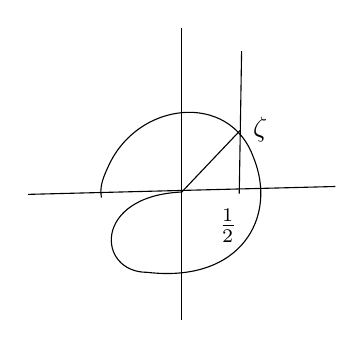
\begin{tikzpicture}[x=1cm,y=1cm]
\draw (-1.95,-.03)--(1.95,.07);
\draw (0,-1.62)--(0,2.08);
\draw (0,0) .. controls (-1.14,-.05) and (-1.08,-1.02) .. (-.44,-1.02) .. controls (.76,-1.16) and (1.22,-.31) .. (.91,.44) .. controls (.61,1.28) and (-.57,1.16) .. (-.94,.31) .. controls (-1.02,.14) and (-1.04,.04) .. (-1.02,-.07);
\draw (.73,-.02)--(.76,1.79);
\draw (0,0)--(.74,.78);
\node[right] at (.79,.79) {$\zeta$};
\node[below] at (.59,-.09) {$\frac12$};
\end{tikzpicture}}

\diagram{\begin{tikzcd}[ampersand replacement=\&,row sep=large,column sep=large]
\Pi_{0,3}^{\mathbb D'} \arrow[r] \arrow[d] \& \Pi_{0,3}^{\mathbb D}=\{\rho,\sigma\mid\rho^3=\sigma^2=1\} \arrow[d,Rightarrow] \\
\deleted{\unsure{\mathbb Z/4\mathbb Z}}\,\inserted{\unsure{\mathbb D'_3}} \arrow[r] \arrow[d] \arrow[ur,phantom,"\unsure{\mathrm{cart}}"{description}] \& \deleted{\unsure{\mathbb Z/2\mathbb Z}}\,\inserted{\unsure{\mathbb D_3}} \arrow[d] \\
\mathbb Z/4\mathbb Z \arrow[r,no head] \arrow[ur,phantom,"\unsure{\mathrm{cart}}"{description}] \& \mathbb Z/2\mathbb Z
\end{tikzcd}}

\margin{$\deleted{\rho\mapsto0,\quad\sigma\mapsto1}$\par
$\rho\mapsto0$\par
$\sigma\mapsto1$}

\margin{\unsure{On remonte} $\rho,\sigma$ en $\deleted{\unsure{\rho,\sigma}}\ \rho',\sigma'$\par
$\rho'=(\rho,2),\quad\sigma'=(\sigma,\deleted{\unsure{2}}\inserted{3})$\par
\unsure{on a}
$\rho'^{\,6}=\sigma'^{\,4}=1,$\par
$\rho'^{\,3}=\sigma'^{\,2}=(\underbrace{1,2\bmod4}_{\omega})$.}

\margin{On vérifie alors aisément que\par
$\mathrm S\ell(2,\mathbb Z)\simeq\{\rho',\sigma'\mid \unsure{\rho'^{\,6}=\sigma'^{\,4}=1},\ \unsure{\rho'^{\,3}=\sigma'^{\,2}}\}$.}

\margin{\figure{\begin{tikzpicture}[x=1cm,y=1cm]
\draw[->] (2.92,3.25) .. controls (2.82,2.34) and (1.35,2.38) .. (1.05,1.46) .. controls (.92,1.12) and (.86,.77) .. (.71,.58);
\draw (0.05,2.24) .. controls (.42,1.64) and (.29,1.03) .. (.21,.96) .. controls (.12,.88) and (.24,.73) .. (.35,.68);
\draw (.59,.98) .. controls (.43,.46) and (.48,.12) .. (.35,-.02) .. controls (.62,.12) and (.63,-.29) .. (.67,-.72);
\end{tikzpicture}}}

Ainsi $\Pi_{0,3}^{\mathbb D'}\simeq\mathrm S\ell(2,\mathbb Z)$ \unsure{apparaît} comme extension de $\Pi_{0,3}^{\mathbb D}$ par $\mathbb Z/2\mathbb Z$, image inverse \deleted{\unsure{de}} l'ext. \inserted{$\mathbb D'_3$} de $\mathbb D_3$ par $\mathbb Z/2\mathbb Z$, ou de l'ext. $\mathbb Z/4\mathbb Z$ de $\mathbb Z/2\mathbb Z$ par $\mathbb Z/2\mathbb Z$, via $\Pi_{0,3}^{\mathbb D}\to\mathbb D_3$ \unsure{resp.} composé $\Pi_{0,3}^{\mathbb D}\to\deleted{\unsure{\mathbb D_3}}\mathbb Z/2\mathbb Z$. \unsure{C'est} une ext. de $\mathbb D'_3$ par un \unsure{gr.} $\simeq\Pi_{0,3}$, \unsure{de base} $\rho_0,\rho_1,\rho_\infty$ \unsure{---}

\margin{15}

\scanpage{17}

\deleted{\diagram{\begin{tikzcd}[ampersand replacement=\&,column sep=small,row sep=large]
\& \vec S(\unsure{X_0|X_\bullet})\simeq G_0 \arrow[dl] \arrow[d] \arrow[dr] \& \\
S(X_0)\simeq G_0/H_S \& A(X_0)\simeq G_0/H_A, \& F(X_0)\simeq G_0/H_F
\end{tikzcd}}}

\deleted{\[
H_S\cap H_A=e,\qquad H_A\cap H_F=e,\qquad H_S\cap H_F=e
\]}

\deleted{\unsure{i.e.|i.a.}
\[
G_0\hookrightarrow G_0/H_S\times G_0/H_A,\qquad
G_0\hookrightarrow G_0/H_A\times G_0/H_F,\qquad
G_0\unsure{\hookrightarrow|\subset}\deleted{\unsure{G_0|H_S}}/H_A\times G_0/H_F
\]}

\deleted{\figure{
\begin{tikzpicture}[x=1cm,y=1cm]
\draw (0,0).. controls (.1,.04) and (.14,.05) .. (.24,.01).. controls (.31,-.02) and (.43,.02) .. (.57,0)--(1.52,0);
\end{tikzpicture}}}

\margin{\uline{\unsure{Cas non orienté}}}

\deleted{Considérons la catégorie des polyèdres (non orientés) de type donné; il y a des foncteurs}

\deleted{\[
\begin{array}{l}
S\\
\vec A\\
F\\
\deleted{\unsure{A|R}}
\end{array}
\]}

\deleted{\diagram{\(\begin{array}{lll}
A_1 & \text{relation d'incidence entre }S\text{ et }A & \text{(}\unsure{\text{arêtes orientées}}\text{ au sens }1\text{)}\\
A_2 & \rule{3.2cm}{0.25pt}\ A\text{ et }F & (\rule{2.8cm}{0.25pt}\ 2)\\
A_3 & \text{rel. d'incidence entre }\unsure{S|B}\text{ et }F &
\end{array}\)}}

\deleted{\[
R=\deleted{\unsure{A_3}}\unsure{\simeq|=}A_1\times_A A_2
\]
\deleted{\unsure{relation} d'incidence entre $S$ et $F$}
\inserted{\unsure{triplets ou drapeaux|triplets de drapeaux} $(s,a,f)$\quad$s\unsure{\leq|<}a<f$.}}

\deleted{\diagram{\begin{tikzcd}[ampersand replacement=\&,row sep=small,column sep=small]
\& R \arrow[dl] \arrow[d] \arrow[dr] \& \\
S\&A\&F
\end{tikzcd}}}

\deleted{\[
\begin{aligned}
A_1&=\operatorname{Im}(R\to S\times A)\\
A_2&=\operatorname{Im}(R\to A\times F)\\
A_3&=\operatorname{Im}(R\to S\times F)
\end{aligned}
\]}

\deleted{$\Omega$ ens des orientations}

\deleted{\[
{A_1}_{\Omega}\simeq\unsure{{A_2}_{\Omega}}\simeq{A_3}_{\Omega}\qquad(
\]}

\[
\mathrm{Pol}_{\unsure{\tau|t}}\qquad
\mathrm{Pol}_{\tau}^{\unsure{\mathrm{or}}}\simeq
\mathrm{Pol}_{\tau}\deleted{\unsure{/\Omega}}\inserted{{}_{/\Omega}}
\]

\margin{16}

\scanpage{18}
\mspage{6}

$S\mathcal T_{1,1}\simeq$ \unsure{image inverse} de $\mathrm S\ell(2,\mathbb Z)$ dans $\unsure{\deleted{\mathrm G\ell}\mathrm S\ell(2,\mathbb R)^{\sim}|\mathrm G\ell(2,\mathbb R)^{\sim}}$
\[
\simeq\{\rho,\sigma\mid\rho^3=\sigma^2\ (=\omega)\}
\]
\margin{\unsure{(}\unsure{élém\textsuperscript{t}|él\textsuperscript{mt}} central}

\[
\mathcal T_{11}=S\mathcal T_{11}/\langle\omega^2\rangle
\]

\[
\begin{array}{ll}
(\mathcal T_{11})_{\mathrm{ab}}\simeq\mathbb Z & (\mathcal T_{11})_{\mathrm{ab}}\simeq\mathbb Z/12\mathbb Z\\[4pt]
\deleted{(\rho,\sigma)} & \\
\rho\longmapsto2 & \rho\longmapsto2\bmod12\\
\sigma\longmapsto3 & \sigma\longmapsto3\bmod12\\
\omega\longmapsto\unsure{6|8} &
\end{array}
\]

\diagram{\begin{tikzcd}[ampersand replacement=\&,row sep=large,column sep=small]
\& 1 \& \& 1 \\
\& \mathcal T_{11} \arrow[u] \arrow[r] \& \deleted{\unsure{\mathcal T_{\mathrm{ab}}}} \arrow[r] \& \mathbb Z/12\mathbb Z \arrow[u] \\
\unsure{\widetilde\omega|\bar\omega}=\omega^{2\deleted{\unsure{4}}} \& S\mathcal T_{11} \arrow[u] \arrow[rr] \arrow[ur,phantom,"\deleted{\text{cartésien}}"{description}] \& \& \mathbb Z \arrow[u] \\
\uline{1} \arrow[u] \& \mathbb Z \arrow[u] \arrow[rr,"\mathrm{id}"] \& \& \mathbb Z \arrow[u,"12"] \\
\& 1 \arrow[u] \& \& 1 \arrow[u]
\end{tikzcd}}

\margin{donc $S\mathcal T_{11}$ se déduit de $\mathcal T_{11}$ par image inverse de l'ext. canonique de $\mathbb Z/12\mathbb Z$ par $\mathbb Z$, via $\mathcal T_{11}\to\mathbb Z/12\mathbb Z$.}

\deleted{une normalisation de $(K,\unsure{K_0|N|k_0})$, \unsure{alors} elle est \unsure{spéciale} : la cat. des rev. étales dans $\unsure{K'_fN|K'_{fN}}$ -- \deleted{\illegible{1}} $\Delta$ \unsure{rev.|i.e.} $\Delta$ top. \unsure{a} une unique normalisation pour laquelle la projection \unsure{est|soit} un \unsure{morphisme} de $\Delta$-complexes \unsure{normalisés}. [Mais attention, \unsure{ça ne marche} \uline{\unsure{pas}} pour \unsure{strictes normalisations} \unsure{$\overline{\mathrm m}$|néc.}\ldots]}

\deleted{\unsure{8.|$\beta$.} \unsure{Groupes|Groupe} et groupoïdes \unsure{fondamentaux|fondamental}. On \unsure{montrera|montre} la relation entre construction top. et construction algébrique.}

\margin{17}

\scanpage{19}

% pencil numeral at the top right corner; no other foliation numeral is visible on this sheet
\margin{8v}

\figure{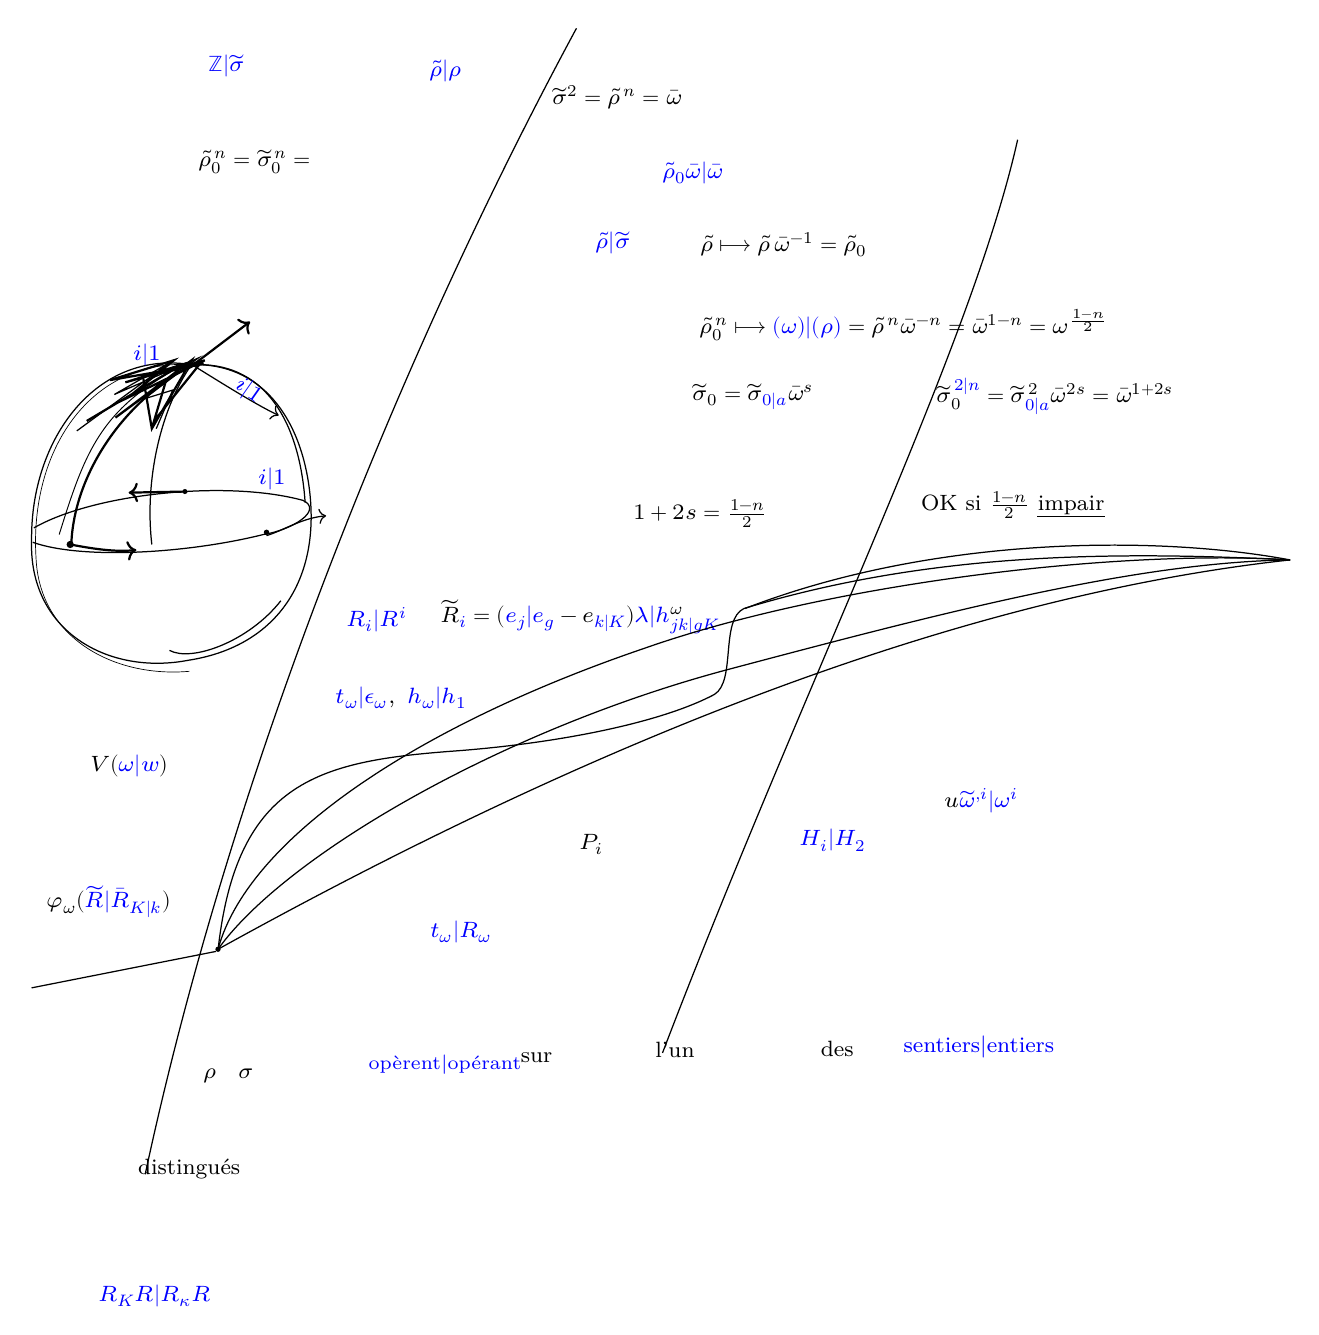
\begin{tikzpicture}[x=.014cm,y=-.014cm,every node/.style={font=\footnotesize,inner sep=0pt},line width=.45pt]
\node[anchor=west] at (385,80) {$\deleted{\unsure{\mathbb Z|\widetilde\sigma}}$};
\node[anchor=west] at (585,85) {$\deleted{\unsure{\widetilde\rho|\rho}}$};
\node[anchor=west] at (376,167) {$\widetilde\rho_0^{\,n}=\widetilde\sigma_0^{\,n}=$};
\node[anchor=west] at (697,109) {$\widetilde\sigma^2=\widetilde\rho^{\,n}=\bar\omega$};
\node[anchor=west] at (796,177) {$\deleted{\unsure{\widetilde\rho_0\bar\omega|\bar\omega}}$};
\node[anchor=west] at (736,241) {$\deleted{\unsure{\widetilde\rho|\widetilde\sigma}}$};
\node[anchor=west] at (831,242) {$\widetilde\rho\longmapsto\widetilde\rho\,\bar\omega^{-1}=\widetilde\rho_0$};
\node[anchor=west] at (830,315) {$\widetilde\rho_0^{\,n}\longmapsto\deleted{\unsure{(\omega)|(\rho)}}=\widetilde\rho^{\,n}\bar\omega^{-n}=\bar\omega^{1-n}=\omega^{\frac{1-n}{2}}$};
\node[anchor=west] at (824,380) {$\widetilde\sigma_0=\widetilde\sigma_{\unsure{0|a}}\bar\omega^s$};
\node[anchor=west] at (1045,380) {$\widetilde\sigma_0^{\,\unsure{2|n}}=\widetilde\sigma_{\unsure{0|a}}^{\,2}\bar\omega^{2s}=\bar\omega^{1+2s}$};
\node[anchor=west] at (770,486) {$1+2s=\frac{1-n}{2}$};
\node[anchor=west] at (1031,478) {OK si $\frac{1-n}{2}$ \uline{impair}};

\draw (328,1085) .. controls (405,726) and (557,346) .. (719,46);
\draw (797,975) .. controls (925,640) and (1077,335) .. (1119,147);

\draw (370,351) .. controls (284,337) and (224,418) .. (225,510) .. controls (222,592) and (294,633) .. (367,619) .. controls (445,607) and (487,549) .. (477,465) .. controls (469,399) and (433,349) .. (370,351);
\draw[line width=.25pt] (371,351) .. controls (277,345) and (223,430) .. (229,526) .. controls (232,599) and (300,635) .. (368,629);
\draw (350,610) .. controls (370,621) and (422,602) .. (451,565);
\draw (227,499) .. controls (281,468) and (401,455) .. (471,474) .. controls (490,483) and (461,501) .. (435,505) .. controls (367,522) and (271,528) .. (226,512);
\draw[line width=.8pt,->] (260,514) .. controls (281,518) and (301,521) .. (320,519);
\draw[line width=.8pt,->] (366,466)--(313,467);
\draw[->] (438,506) .. controls (454,501) and (470,490) .. (492,488);
\fill (260,514) circle[radius=3.3];
\fill (438,503) circle[radius=2.5];
\fill (364,466) circle[radius=2.3];
\draw (334,514) .. controls (327,454) and (343,389) .. (370,351);
\draw[line width=.8pt] (261,514) .. controls (263,455) and (303,388) .. (370,351);
\draw[line width=.35pt] (250,505) .. controls (274,428) and (288,390) .. (365,350);
\draw[line width=.8pt,->] (369,353)--(423,312);
\draw[->] (372,352) .. controls (398,368) and (428,387) .. (449,397);
\draw (377,351) .. controls (437,351) and (468,403) .. (473,476);
\node at (330,342) {$\unsure{i|1}$};
\node[rotate=-35] at (422,375) {$\unsure{i|1}$};
\node at (443,455) {$\unsure{i|1}$};
\draw[line width=.8pt] (275,402)--(361,351)--(310,367)--(382,347)--(312,381)--(354,347)--(296,365)--(377,351)--(336,402)--(347,365)--(301,399)--(370,347)--(334,409)--(326,362)--(381,350);
\draw (266,411)--(352,348)--(300,378)--(376,345)--(327,382)--(353,374)--(338,409);

\node[anchor=west] at (510,582) {$\unsure{R_i|R^i}$};
\node[anchor=west] at (595,580) {$\widetilde R_{\unsure{i}}=(\unsure{e_j|e_g}-e_{\unsure{k|K}})\unsure{\lambda|h}^{\omega}_{\unsure{jk|gK}}$};
\node[anchor=west] at (500,653) {$\unsure{t_\omega|\epsilon_\omega},\ \unsure{h_\omega|h_1}$};
\node[anchor=west] at (278,715) {$V(\unsure{\omega|w})$};
\node[anchor=west] at (238,838) {$\varphi_\omega(\unsure{\widetilde R|\bar R}_{\unsure{K|k}})$};
\node[anchor=west] at (721,786) {$P_i$};
\node[anchor=west] at (586,865) {$\deleted{\unsure{t_\omega|R_\omega}}$};
\node[anchor=west] at (921,782) {$\deleted{\unsure{H_i|H_2}}$};
\node[anchor=west] at (1052,746) {$u\unsure{\widetilde\omega^{,i}|\omega^i}$};

\draw (225,916)--(392,883);
\fill (394,881) circle[radius=2.4];
\draw (394,882) .. controls (411,727) and (487,710) .. (612,701) .. controls (702,694) and (795,676) .. (844,650) .. controls (864,638) and (849,582) .. (871,572) .. controls (1039,521) and (1205,520) .. (1366,528);
\draw (394,881) .. controls (422,778) and (581,676) .. (781,608) .. controls (949,549) and (1211,518) .. (1366,528);
\draw (394,881) .. controls (454,797) and (649,683) .. (854,628) .. controls (1057,574) and (1228,530) .. (1366,528);
\draw (394,881) .. controls (721,700) and (1056,562) .. (1366,528);
\draw (872,572) .. controls (1045,505) and (1249,506) .. (1366,528);

\node[anchor=west] at (380,996) {$\rho\quad\sigma$};
\node[anchor=west,font=\scriptsize] at (530,986) {\unsure{opèrent|opérant}};
\node[anchor=west] at (668,979) {sur};
\node[anchor=west] at (790,972) {l'un};
\node[anchor=west] at (940,971) {des};
\node[anchor=west] at (1015,970) {\unsure{sentiers|entiers}};
\node[anchor=west] at (321,1080) {distingués};
\node[anchor=west] at (285,1195) {$\deleted{\unsure{R_KR|R_\kappa R}}$};
\end{tikzpicture}}
\scanpage{20}
\figure{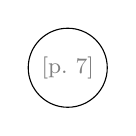
\begin{tikzpicture}
\node[draw,circle,inner sep=3pt] {\mspage{7}};
\end{tikzpicture}}

\diagram{\begin{tikzcd}[ampersand replacement=\&,column sep=1.6em,row sep=2.8em]
\&\&
\begin{gathered}
\widetilde\rho=(\rho_0,2)=(\rho,2)\\
\widetilde\sigma=(\sigma_0,3)=(\sigma,3)
\end{gathered}
\arrow[d, bend right=20]
\&
\begin{gathered}
\deleted{\unsure{\Pi_{0,3}^{D}}}\\[-2pt]
\inserted{\text{\uline{\unsure{identifié à}}}}\\[-2pt]
\inserted{\unsure{S\mathcal T_{11}\times_{\Pi_{0,3}^{D}}\mathbb Z/12\mathbb Z}}
\end{gathered}
\arrow[d]
\&
\begin{gathered}
\rho_0=(\rho,\dot 2)\\[-2pt]
\unsure{\Pi_{0,3}}\\[-2pt]
\sigma_0=(\sigma,\dot 3)=(\sigma,-1)
\end{gathered}
\arrow[d]
\&\\
\unsure{0|1}\arrow[r,dash]\&
\mathbb Z\arrow[r,dash,"1\unsure{-|\mapsto}\overline\omega=\omega^2"]\arrow[dd,equal]\&
S\mathcal T_{11}\arrow[r,Rightarrow]\arrow[dd,"\substack{\widetilde\rho\mapsto\deleted{\unsure{4}}2\\\widetilde\sigma\mapsto3}"']
\arrow[ddr,phantom,"\text{Cart}"]\&
\mathcal T_{11}\arrow[r,Rightarrow]\arrow[dr,leftrightarrow]\arrow[dd,"\substack{\rho_0\mapsto\dot 2\\\sigma_0\mapsto\dot 3}"']
\&\Pi_{0,3}^{\prime D}\arrow[dr,"\text{can}"]\arrow[dd,"\substack{\rho\mapsto2\\\sigma\mapsto3}"{pos=.25,xshift=2pt}]
\arrow[dl,phantom,"\text{cart}" description]\&\\
\&\&\&{}\&
|[xshift=-3em]|\mathbb D'_3\arrow[r,"\text{cart}"{pos=.75}]\arrow[dd]
\&\mathbb D_3\arrow[dd,"\text{can}"]\\
1\arrow[r,dash]\&\mathbb Z\arrow[r,"12"]\&\mathbb Z\arrow[r,"\text{can}"]\&
\mathbb Z/12\mathbb Z\arrow[r,"\text{can}"]\arrow[dr,"\text{can}"']
\&\mathbb Z/6\mathbb Z\arrow[dr,"\text{can}"]
\arrow[d,phantom,"\text{\uline{Cart}}"'{pos=.25,xshift=-3em}]
\arrow[dr,phantom,"\text{\uline{cart}}"{description,xshift=-1.5em,yshift=.5em}]\&\\
\&\&\&\&\mathbb Z/4\mathbb Z\arrow[r,leftrightarrow,"\text{can}"]\&\mathbb Z/2\mathbb Z
\end{tikzcd}}

\margin{\unsure{pour} $\mathcal T_{11}$ \unsure{identifié à}
$\Pi_{0,3}^{D}\times_{\mathbb Z/2\mathbb Z}\mathbb Z/4\mathbb Z$}

\unsure{A-t-on} \unsure{bien}\quad
$\bigm|\quad S\mathcal T_{11}\simeq S\Pi_{0,3}^{D}$ ??

il semblerait plutôt, pourtant
\[
\deleted{\unsure{\mathcal T_{11}}}\quad
PM_{11}\simeq
\left(\underbrace{T^*U_{0,3}}_{\substack{\text{fibré}\\\text{\uline{tangent}}}},\mathfrak S_3\right)
\]
\inserted{(et \uline{non} $\unsure{PU_{0,3}}$ !!)}

\[
\text{donc}\quad \mathcal T_{11}\simeq\pi_1(T^*U_{0,3},\mathfrak S_3)\ \ldots
\]
\margin{19}

\scanpage{21}
% Trois longs traits obliques au crayon, terminés chacun en crochet, traversent tout le feuillet : rature d'ensemble.
% Les ratures à l'encre (ligne « Op. ext. … », « compatible avec l'op. ext. », E corrigé en F, 1 et π_1 de la dernière suite) restent marquées à l'intérieur.
\deleted{
\[
\pi\qquad l_1\ \cdots\ l_n
\]

\diagram{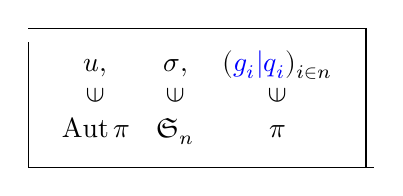
\begin{tikzpicture}
\node[inner sep=7pt] (p) {$\begin{array}{ccc}
u,&\sigma,&(\unsure{g_i|q_i})_{i\in n}\\
\rotatebox{90}{$\in$}&\rotatebox{90}{$\in$}&\rotatebox{90}{$\in$}\\
\operatorname{Aut}\pi&\mathfrak S_n&\pi
\end{array}$};
\draw (p.north west) -- (p.north east) -- (p.south east);
\draw ([yshift=-5pt]p.north west) -- (p.south west) -- ([xshift=3pt]p.south east);
\end{tikzpicture}}
\diagram{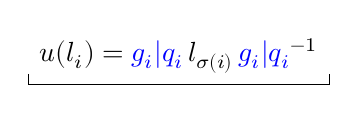
\begin{tikzpicture}
\node[inner sep=4pt] (u) {$u(l_i)=\unsure{g_i|q_i}\,l_{\sigma(i)}\,\unsure{g_i|q_i}^{-1}$};
\draw ([yshift=4pt]u.south west) -- (u.south west) -- (u.south east) -- ([yshift=4pt]u.south east);
\end{tikzpicture}}

\diagram{\begin{tikzcd}[ampersand replacement=\&,column sep=1.5em]
1\arrow[r,dash]\&\pi_1(\operatorname{Aut}(X)\arrow[r]\&\mathbb Z^n\arrow[r]\&S\mathcal T\arrow[r]\&\mathcal T\arrow[r,dash]\&\mathfrak S_n\arrow[r,dash]\&1
\end{tikzcd}}

\diagram{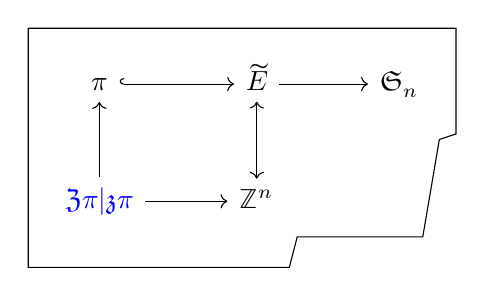
\begin{tikzpicture}
\node[inner sep=9pt] (b) {\begin{tikzcd}[ampersand replacement=\&,column sep=3em,row sep=2.5em]
\pi\arrow[r,hook]\&\widetilde E\arrow[r]\arrow[d,leftrightarrow]\&\mathfrak S_n\\
\unsure{\mathfrak Z\pi|\mathfrak z\pi}\arrow[u]\arrow[r]\&\mathbb Z^n\&{}
\end{tikzcd}};
\draw (b.north west) -- (b.north east) -- ([yshift=2pt]b.east) -- ([xshift=-6pt]b.east)
 -- ([xshift=-12pt,yshift=5pt]b.south east) -- ([xshift=0.7cm,yshift=5pt]b.south)
 -- ([xshift=0.6cm,yshift=-6pt]b.south) -- ([yshift=-6pt]b.south west) -- (b.north west);
\end{tikzpicture}}

\diagram{\begin{tikzcd}[ampersand replacement=\&,column sep=2.3em,row sep=1.8em]
\&\&1\&\&\\
1\arrow[r]\&\underbrace{S\operatorname{Aut}^{+}(X)}\arrow[r]\arrow[d,"\simeq"]\&
\operatorname{Aut}^{+}(X)\arrow[u]\arrow[r,dash]\&\operatorname{Aut}^{+}(\partial X)\arrow[r,dash]\&1\\
\&\uline{S\mathcal T}\&\operatorname{Aut}^{+}_{!}(\widetilde X)\arrow[u]\&\uline{\mathfrak S_n\cdot\mathbb T^n}\arrow[u,"\simeq"]\&\\
\&\&\pi\arrow[u]\&\&\\
\&\&1\arrow[u]\&\&
\end{tikzcd}}

\diagram{\begin{tikzcd}[ampersand replacement=\&,column sep=1.6em]
1\arrow[r,dash]\&\underbrace{\pi_1\operatorname{Aut}^{+}(X)}_{0\ \text{ou}\ \mathbb Z}\arrow[r,Rightarrow]\&\mathbb Z^n\arrow[r,dash]\&S\mathcal T\arrow[r,dash]\&\mathcal T\arrow[r,dash]\&\mathfrak S_n\arrow[r,dash]\&1
\end{tikzcd}}

\diagram{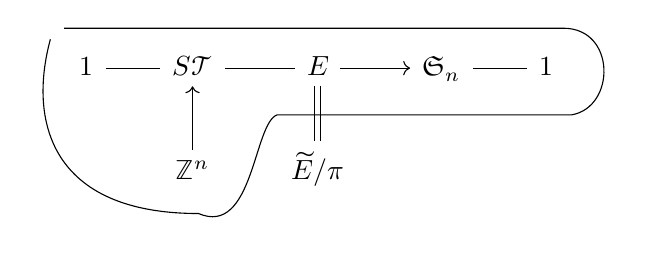
\begin{tikzpicture}
\node[inner sep=6pt] (e) {\begin{tikzcd}[ampersand replacement=\&,column sep=2em,row sep=1.8em]
1\arrow[r,dash]\&S\mathcal T\arrow[r,dash]\&E\arrow[r]\arrow[d,equal]\&\mathfrak S_n\arrow[r,dash]\&1\\
\&\mathbb Z^n\arrow[u]\&\widetilde E/\pi\&\&{}
\end{tikzcd}};
\draw ([xshift=5pt]e.north west) -- ([xshift=-7pt]e.north east)
 .. controls ([xshift=12pt]e.north east) and ([xshift=12pt,yshift=-1cm]e.north east) .. ([xshift=-4pt,yshift=-1.1cm]e.north east)
 -- ([xshift=-0.5cm,yshift=-1.1cm]e.north)
 .. controls ([xshift=-0.8cm,yshift=-1.2cm]e.north) and ([xshift=-0.8cm,yshift=-0.3cm]e.south) .. ([xshift=-1.5cm]e.south)
 .. controls (e.south west) and ([xshift=-8pt]e.west) .. ([yshift=-4pt]e.north west);
\end{tikzpicture}}

\diagram{\begin{tikzcd}[ampersand replacement=\&,column sep=2.4em,row sep=2em]
1\arrow[r,dash]\&\unsure{\widetilde F|\widehat F}\arrow[r,dash]\arrow[d]\&\widetilde A\arrow[r,dash]\arrow[d]\&\widetilde G\arrow[d]\&\\
1\arrow[r,dash]\&\substack{\deleted{\unsure{E}}\inserted{F}\\\text{discret}}\arrow[r]\&A\arrow[r]\&G\arrow[dr]\&
\bigl(=\mathfrak S_n\unsure{\ast|\cdot}\mathbb T^n\bigr)\\
\&\&\&\&1
\end{tikzcd}}

\deleted{\unsure{Op.} ext. de $\pi_0$ sur $F$}

\diagram{\begin{tikzcd}[ampersand replacement=\&,column sep=3.8em,row sep=2.3em]
\pi_1(G)=\pi_1\arrow[r]\arrow[dr,bend right=20,"\substack{\text{\unsure{compatible}}\\\text{avec }\pi_0}"']\&F\arrow[d,phantom,"\cup" description]\\
\&\unsure{\mathfrak Z(F)|\mathfrak z(F)}
\end{tikzcd}}
\inserted{\unsure{central}}

$\pi_0(G)=\pi_0$ opère \unsure{extérieurement} sur $F$
\quad donc opère sur $\unsure{\mathfrak Z(F)|\mathfrak z(F)}$

\diagram{$\begin{array}{cc}
\pi_0&\pi_1\\
\multicolumn{2}{c}{\text{op.}}
\end{array}$}
\deleted{\unsure{compatible} avec l'op. ext.}

\diagram{\begin{tikzcd}[ampersand replacement=\&,column sep=2.4em,row sep=1.7em]
1\arrow[r,dash]\&F\arrow[r]\&E\arrow[r]\arrow[d,equal]\&\pi_0\arrow[r,dash]\&1\\
\&\&\pi_0(\widetilde A)\&\&{}
\end{tikzcd}}
\figure{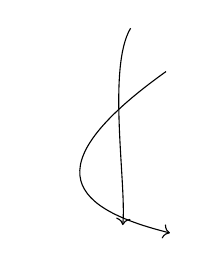
\begin{tikzpicture}[x=1cm,y=1cm]
\draw[->] (0.3,2.5) .. controls (0.0,2.0) and (0.25,0.5) .. (0.2,0);
\draw[->] (0.75,1.95) .. controls (-1.0,0.7) and (-0.4,0.2) .. (0.8,-0.1);
\end{tikzpicture}}

\diagram{\begin{tikzcd}[ampersand replacement=\&,column sep=1.6em]
1\arrow[r,dash]\&\pi_1(A)\arrow[r,dash]\&\pi_1\arrow[r]\&\unsure{F}\arrow[r]\&\underbrace{\pi_0(A)}\arrow[r]\&\substack{\unsure{\pi_0|\pi_\infty}\\ /}\arrow[r,dash]\&1
\end{tikzcd}}

\diagram{\begin{tikzcd}[ampersand replacement=\&,column sep=1.7em,row sep=1.5em]
\deleted{\unsure{1}}\arrow[r,dash]\&\deleted{\unsure{\pi_1}}\arrow[r,dash]\&F\arrow[r,dash]\&\pi_0(\widetilde A)\arrow[r]\arrow[d,equal]\&\pi_0\arrow[r]\&1\\
\&\&\&E\&\&{}
\end{tikzcd}}
}
\margin{20}

\scanpage{22}
% blank
\margin{21}

\scanpage{23}
A)\quad \uline{Lemme}\quad
$S$ schéma \deleted{\unsure{satisfaisant|strictement}}
régulier intègre tel que $\operatorname{Pic}(S)=0$,
car. du point générique $\ne2$ Alors \deleted{$\unsure{H^1}$}
\[
H^1(U_{0,3},\mathfrak S_3;\mathbb G_m]\simeq\mathbb Z/6\mathbb Z
\]
(\deleted{\unsure{résiduelle}}\inserted{\unsure{pt gén.|si gén.}} est $2$, on trouve $\mathbb Z/3\mathbb Z$)

\margin{\uline{\unsure{Dém}}\quad on utilise suite exacte
\diagram{\begin{tikzcd}[ampersand replacement=\&,column sep=1.3em,row sep=2em]
0\arrow[r]\&H^1(\mathfrak S_3,H^0(U_{0,3},\mathbb G_m)\arrow[r]\&H^1(\text{mixte})\arrow[dll]\&{}\\
H^0\bigl(\mathfrak S_3,\underbrace{H^1(U_{0,3};\mathbb G_m)}_{0}\bigr)\&\&\&{}
\end{tikzcd}}
et
\diagram{\begin{tikzcd}[ampersand replacement=\&,column sep=1.3em]
0\arrow[r]\&H^0(S,\mathbb G_m)\arrow[r]\&H^0(U_{0,3},\mathbb G_m)\arrow[r]\&\unsure{h_1(V(J))|h^1(V(J))}\arrow[r]\&0
\end{tikzcd}}}

\unsure{Je} dis que si \inserted{le schéma}
$\deleted{\unsure{U_{0,3}}}\inserted{\Sigma_J}$ est défini comme $\mathbb P(V_J)$, \unsure{i.e.}
\diagram{\begin{tikzcd}[ampersand replacement=\&,column sep=2.8em]
0\arrow[r,dash]\&V_J\arrow[r]\&\mathcal O^J\arrow[r]\&\mathcal O\arrow[r,dash]\&0
\end{tikzcd}}
alors le fibré \unsure{principal}
\[
P\Sigma_J=\check V(\mathcal O_{\Sigma_J}(1))^{*}
\]
est un générateur du
$H^1(\deleted{\unsure{U_{0,3}}}\inserted{\Sigma_J^*},
\deleted{\unsure{\mathfrak S_3}}\inserted{\mathfrak S_J};\mathbb G_m)$.

Je vais d'abord \unsure{trouver} une trivialisation de
\[
\uline{\mathcal O}(1)^{\otimes6}=\mathcal O(6)\simeq
\unsure{\mathcal T^{\otimes3}(\omega)|\mathcal J^{\otimes3}(\omega)},
\]
\deleted{donc} \inserted{en fait} une section de $\mathcal O(6)$
\inserted{sur $\overline\Sigma$ \unsure{tout entier}}
(qui \deleted{\unsure{ne s'annule que}}
\inserted{\unsure{est}, \unsure{inversible}} sur $\Sigma^*$.
On \deleted{\unsure{prenant}} a
\[
\Gamma(\Sigma_J,\mathcal O(6))\simeq\operatorname{Sym}^{6}V_J
\]
et on prendra
\[
\begin{gathered}
\unsure{\varphi|\Delta}\in\Gamma(\Sigma_J,\mathcal O(6)),\qquad
\unsure{\varphi|\Delta}
=\deleted{\unsure{\sum_{i\in J}}}
-\prod_{\substack{i,j\in J\\i\ne j}}(e_i-e_j)\\
=\prod_{i\in J}\underbrace{(e_j-e_h)}_{J=\{i,j,h\}}^{2}.
\end{gathered}
\]
Ainsi, sur $\deleted{\unsure{U_J}}\inserted{\Sigma_J^{*}}$, le groupe \unsure{structural|structurel}
\deleted{\unsure{de}}
$\mathbb G_m$ de $P\Sigma_J^{*}$ est réduit \unsure{à|:} $\mu_6$.

\uline{NB}\quad Sauf erreur, on a
\[
\deleted{\unsure{\operatorname{Sym}}}\quad
\operatorname{Sym}^{*}(V_J)^{\mathfrak S_3}\simeq
\mathcal O\bigl(\unsure{\gamma_2|\varphi_2},\unsure{\gamma_3|\varphi_3}\bigr)
/(2\gamma_3^2-\gamma_2^3)
\]
\[
\left\{\begin{aligned}
\gamma_2&=\sum_{i\in J}(e_j-e_h)^2\\
\gamma_3&=\prod_{i\in J}(e_j\unsure{-|+}e_h-2e_i)
\end{aligned}\right.
\qquad\text{et}\quad\Delta=\gamma_2^3
\]
\margin{22}

\scanpage{24}
% not manuscript: tract imprimé « Parler Femmes à propos de “PLURIELLES” », avec une longue rature diagonale.
\margin{23}

\scanpage{25}
B)

\deleted{\unsure{Si} $2$ \unsure{inversible}, on \unsure{aura} \unsure{donc}}
\[
\deleted{\operatorname{Sym}^{*}(\unsure{V_J|W_J})^{\mathfrak S_{\unsure{J|3}}}\simeq\mathcal O[}
\]
\deleted{\unsure{Remarque}}

Comme $\gamma_2$ s'annule en \deleted{\unsure{les}} $P_\omega$,
$\gamma_3$ en les $Q_i$, il s'ensuit qu'il n'y a pas de section invariante
d'un $\mathcal O(n)^*$ \deleted{\unsure{pour}} sur
$\Sigma_J^{*}$ \deleted{\unsure{en degré} $<$}
pour $n\le6$, donc que l'ordre de
$\operatorname{cl}(\mathcal O(1))$ dans
$H^1(\Sigma_J,\mathfrak S_J;\mathbb G_m)$ est bien $6$,
ce qui \unsure{prouve} que $\mathcal O(1)$ est un générateur du
$\unsure{H^1}$ mixte.
\margin{24}
\scanpage{26}
% not manuscript: feuillet dactylographié « Sciences de l’homme », « Energie », « Mécanique et industries de transformation », « Recherches sur les milieux tropicaux et sub-tropicaux » ; pagination imprimée « - 4 - ».
\margin{25}

\scanpage{27}
% Étiquette imprimée, oblique et à l'envers sur le feuillet.
\begin{flushleft}
MR LE PROFESSEUR GROTHENDIECK ALEX.\\
MATHEMATIQUES\hfill 5
\end{flushleft}

\diagram{\begin{tikzcd}[ampersand replacement=\&,column sep=huge]
\mathbb D'_3 \arrow[r] \& \mathbb D_3
\end{tikzcd}}

\margin{\figure{\begin{tikzpicture}[x=1cm,y=1cm]
\draw (0,0) .. controls (.1,.14) and (.25,.13) .. (.48,.03);
\end{tikzpicture}}}

\diagram{\begin{tikzcd}[ampersand replacement=\&,column sep=large,row sep=large]
PM_{11}(2^{\sim})\overset{?}{\simeq}PU_{0,3}
  \arrow[r,very thick] \arrow[d,leftrightarrow]
\& PM_{11}(2)\simeq TU_{0,3} \arrow[d]\\
U_{0,3}\simeq M_{11}(\unsure{\widetilde{2}^{\sim}|2^{\sim}})
  \arrow[r,very thick]
\& \begin{gathered}(U_{0,3},\{1,\omega\})\\[-2pt]{}\simeq M_{11}(\unsure{2})\end{gathered}
\arrow[ul,phantom,"\mathrm{cart}" description]
\end{tikzcd}}

\[
\deleted{\unsure{x}\longrightarrow\unsure{x^2\wedge\omega_0}}
\]
\[
\unsure{H^1}(TU_{03},\mathbb D_3;\mu_2)
\]

\diagram{\begin{tikzcd}[ampersand replacement=\&,column sep=small,row sep=large]
M_{11}(2^{\sim}) \arrow[rr]
  \arrow[dr,"{\deleted{\unsure{\mathcal D/\Pi_{0,3}|\mathbb Z/2\,\Pi_{0,3}}}}"']
\& \& M_{11}(2)\unsure{-|'} \arrow[dl] \arrow[d,leftrightarrow] \& \phantom{M}\\
\& M_{11} \arrow[d] \& M_{11}(2)' \arrow[dl] \& \\
\phantom{M}\arrow[rrruu,dashed,no head,shorten <=-10pt,shorten >=-10pt]
\& M'_{11} \& \&
\end{tikzcd}}

\diagram{\begin{tikzcd}[ampersand replacement=\&,column sep=small,row sep=large]
U_{03} \arrow[rr,"{\{1,\omega\}}"] \arrow[dr,"{\mathbb D'_3}"']
\& \& (U_{0,3},\{1,\omega\}) \arrow[dl,"{\mathbb D_3}"'] \arrow[d,"{\unsure{\mathrm{gerbe}}}"] \& \phantom{U}\\
\& (U_{0,3},\mathbb D'_3) \arrow[d,"{\unsure{\mathrm{gerbe}}}"']
\& (U_{03}) \arrow[dl,"{\mathbb D_3}"] \& \\
\phantom{U}\arrow[rrruu,dashed,no head,shorten <=-12pt,shorten >=-12pt]
\& (U_{0,3},\mathbb D_3) \& \&
\end{tikzcd}}

\diagram{\begin{tikzcd}[ampersand replacement=\&,column sep=small,row sep=large]
\begin{gathered}(\mathcal D,\Pi_{03})\\[-2pt]{}\simeq\mathcal D/\Pi_{03}\end{gathered}
 \arrow[rr,very thick,"{\mathrm{gal}}","{\{1,\omega\}}"']
 \arrow[dr,"{\begin{gathered}\mathrm{gal}\\\mathbb D'_3\end{gathered}}"']
\& \& (\mathcal D,\Pi_{03}\times\{1,\omega\})
 \arrow[dl,"{\begin{gathered}\mathrm{gal}\\\mathbb D_3\ \deleted{\unsure{\{1,\omega\}}}\end{gathered}}"']
 \arrow[d,"{\unsure{2\text{-}\uline{\mathrm{gerbe}}}}"] \& \phantom{D}\\
\& (\mathcal D,\unsure{\mathrm{Sl}(2,\mathbb Z)})
 \arrow[d,"{\unsure{2\text{-}\mathrm{gerbe}}}"']
\& (\mathcal D,\Pi_{03}) \arrow[dl,"{\begin{gathered}\mathrm{gal}\\\mathbb D_3\end{gathered}}"] \& \\
\phantom{D}\arrow[rrruu,dashed,no head,shorten <=-12pt,shorten >=-12pt]
\& (\mathcal D,\unsure{\mathrm{Sl}(2,\mathbb Z)}') \& \&
\end{tikzcd}}

\margin{26}

\scanpage{28}
% not manuscript: avis dactylographié, à l’envers, de soutenance d’une thèse de doctorat de 3ème cycle, « Algèbres de Rees », YOON Suk-Im, Montpellier, le 26 février 1982 ; soutenance prévue le 4 MARS 1982 à 15h.
\margin{27}

\scanpage{29}

\deleted{\diagram{\begin{tikzcd}[ampersand replacement=\&,column sep=small,row sep=large]
\& \& {}\arrow[r,"{\unsure{''|1}}"]
\& \mathrm{Sl}(2,\mathbb Z)\arrow[r]\arrow[d]
\& \Pi_{0,3}^{D}\arrow[d] \& \\
\& \unsure{\widetilde\varepsilon|\widetilde E}\arrow[rr]
  \arrow[ddl]\arrow[dr,dashed]
\& \& \mathbb D_3\mathop{\times}\limits_{\mathbb Z/2\mathbb Z}
       \mathbb Z/\unsure{12}\mathbb Z
       \simeq\mathbb D'_3\mathop{\times}\limits_{\mathbb Z/\unsure{2}\mathbb Z}
       \mathbb Z/6\mathbb Z
       \arrow[r]\arrow[dd,very thick]\arrow[d,dashed]
\& \mathbb D_3\mathop{\times}\limits_{\mathbb Z/2\mathbb Z}
       \mathbb Z/6\mathbb Z=\unsure{\varepsilon|E}
       \arrow[dd]\arrow[dr] \& \\
\& \& \mathbb Z\arrow[r,no head]\arrow[ddl,dashed,leftrightarrow,very thick]
\& \mathbb Z/12\mathbb Z\arrow[rr,dashed,"{\mathrm{can}}"]
       \arrow[dd,dashed,"{\mathrm{can}}"'{pos=.2}]
\& \& \mathbb Z/6\mathbb Z\arrow[ddl,"{\mathrm{can}}"]\\
\unsure{\widetilde{\mathbb D}_3^{*}|\widetilde{\mathbb D}'_3}
 \arrow[rrr,very thick]\arrow[dr]
\& \& \& \mathbb D'_3\arrow[r,very thick]\arrow[d,very thick]
\& \mathbb D_3\arrow[d,"{\mathrm{can}}"] \& \\
\& \mathbb Z\arrow[rr] \& \& \mathbb Z/4\mathbb Z\arrow[r,"{\mathrm{can}}"]
\& \mathbb Z/2\mathbb Z \&
\end{tikzcd}}}

\figure{
\begin{tikzpicture}[x=1cm,y=1cm]
\draw (0,.06) .. controls (2,.16) and (9,-.05) .. (13,0);
\end{tikzpicture}}

\diagram{\begin{tikzcd}[ampersand replacement=\&,column sep=small,row sep=large]
\unsure{\mathbb Z_{(\omega/2)}}\arrow[r]\arrow[d,very thick]
\& \widetilde\Pi_{0,3}^{\unsure{\circ}}
   \deleted{\unsure{\widetilde\Pi_{0,3}}}\arrow[rr,very thick]\arrow[d]
\& \& \Pi_{0,3}\arrow[d,leftrightarrow,bend left=12]
\& \& \& \\
\mathbb Z_{(\omega)}\arrow[r,very thick]\arrow[d,equal]
\& \widetilde\Pi_{0,3}^{\unsure{'}}\arrow[rr]\arrow[d,very thick]
\& \& \Pi'_{0,3}=\Pi_{0,3}\times\{1,\omega\}
   \arrow[rr]\arrow[d,bend right=12]
\& \& \Pi_{03}\arrow[d,bend right=18] \& \\
\mathbb Z\arrow[r,very thick]\arrow[d,equal]
\& \widetilde{\mathrm{Sl}}(2,\mathbb Z)=\widetilde\Pi_{0,3}^{D}
   \arrow[rr]\arrow[d]
\& \& \mathrm{Sl}(2,\mathbb Z)\arrow[rr]\arrow[d,very thick]\arrow[ddr]
\& \& \Pi_{0,3}^{D}\arrow[d]\arrow[ddr] \& \\
\mathbb Z\arrow[r]\arrow[dd,equal]
\& \widetilde{\mathbb D}_3\arrow[rr]\arrow[dd]
\& \& \begin{gathered}\mathbb D'''_3\\\margin{3}\end{gathered}\arrow[rr,"2"]\arrow[dr,"3"']\arrow[dd,"3"']
\& \& \begin{gathered}\mathbb D''_3\\\margin{\unsure{12|10}}\end{gathered}\arrow[dr,"3"]\arrow[dd,"3"'{pos=.72}] \& \\
\& \& \& \& \mathbb D'_3\arrow[rr,"2"{pos=.75}]\arrow[dd,"3"{pos=.77}]
\& \& \mathbb D_3\arrow[dd,"3"]\\
\mathbb Z\arrow[r,"12"]
\& \mathbb Z\arrow[rr]
\& \& \mathbb Z/12\mathbb Z\arrow[rr,leftrightarrow,"2"]\arrow[dr,"3"']
\& \& \mathbb Z/6\mathbb Z\arrow[dr,"3"] \& \\
\& \& \& \& \mathbb Z/4\mathbb Z\arrow[rr,"2"] \& \& \mathbb Z/2\mathbb Z
\end{tikzcd}}
\margin{\unsure{fond|bon}}

\diagram{\begin{tikzcd}[ampersand replacement=\&,column sep=large,row sep=large]
1\arrow[r,no head]
\& \mathbb Z\arrow[r,no head]\arrow[d,very thick,"{\begin{gathered}4\\\unsure{4}\end{gathered}}"]
\& \widetilde\Pi_{0,3}^{D}\arrow[r,no head]\arrow[d,no head]
\& \Pi_{0,3}^{D}\arrow[r]\arrow[d,no head]
\& 1\\
1\arrow[r,no head]
\& \mathbb Z\arrow[r,no head]
\& \widetilde\Pi_{0,3}^{D}(4)\arrow[r]
\& \Pi_{0,3}^{D}\arrow[r,very thick]
\& 1
\end{tikzcd}}

\figure{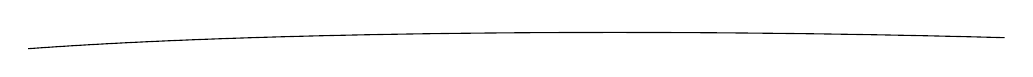
\begin{tikzpicture}[x=1cm,y=1cm]
\draw (0,0) .. controls (3,.22) and (8,.26) .. (12.4,.14);
\end{tikzpicture}}

\diagram{\begin{tikzcd}[ampersand replacement=\&,column sep=large,row sep=large]
\& \& \widetilde\Pi_{0,3}^{D}
\& \Pi_{0,3}^{D}\arrow[r,no head] \& 1\\
1\arrow[r]
\& \overset{\omega}{\mathbb Z}\arrow[r]
\& \widetilde\Pi_{0,3}^{D}(4)\arrow[r]
\& \Pi_{0,3}^{D}\times\mathbb Z/4\mathbb Z\arrow[u]\arrow[r,no head]
\& 1\\
1\arrow[r,no head]
\& \mathbb Z\arrow[r]
\& ?\arrow[r]
\& \unsure{\mathrm{Sl}(2,\mathbb Z)}\arrow[u]\arrow[r,no head]
\& 1
\end{tikzcd}}

\margin{28}

\scanpage{30}
% Secteur supérieur : un long trait courbe au crayon, terminé en crochet, descend de « par les e_i-e_j » vers le bas à gauche ;
% il traverse les trois premières lignes, la suite Z — Π̃_03 — Π_03 → 1 et la formule V(ω) ≃ V, barrées ici en bloc.
\deleted{
$V_J\deleted{\unsure{\simeq}}\inserted{=\unsure{\Gamma(X,\uline{\mathcal O}(1))}}
\deleted{e_i-e_j}$ \unsure{engendré} par les $e_i-e_j$

\deleted{$\unsure{\Pi(e_i-e_j)|P(e_i-e_j)}$}
\unsure{comment} ces \unsure{sections} \unsure{sont} elles
\unsure{permutées} entre elles
}

\figure{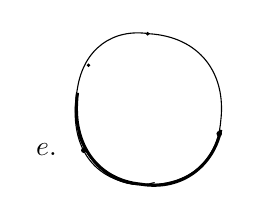
\begin{tikzpicture}[x=1cm,y=1cm]
\draw (0,.95) .. controls (.64,.91) and (.98,.45) .. (.91,-.15)
 .. controls (.86,-.78) and (.36,-1.04) .. (-.25,-.95)
 .. controls (-.83,-.83) and (-1.02,-.33) .. (-.91,.26)
 .. controls (-.83,.76) and (-.46,1.02) .. (0,.95);
\draw[line width=1.1pt] (-.91,.2) .. controls (-1,-.48) and (-.63,-.91) .. (-.11,-.96)
 .. controls (.43,-1.05) and (.82,-.71) .. (.91,-.27);
\draw (-.9,-.33) .. controls (-.72,-.82) and (-.31,-1.05) .. (.07,-.94);
\fill (-.02,.95) circle (.025);
\fill (-.77,.55) circle (.024);
\fill (-.83,-.53) circle (.035);
\fill (.89,-.32) circle (.035);
\node[left] at (-1.04,-.52) {$e.$};
\end{tikzpicture}}

\[
\deleted{e_i-e_j\qquad\unsure{\mathcal O(6)|\mathcal O(1)}}
\qquad e_i-e_j=
\]
\[
\unsure{\xi_i}.
\]

\diagram{\begin{tikzcd}[ampersand replacement=\&,column sep=small,row sep=small]
\unsure{\uline{\mathcal O}_x(1)|\uline{\mathcal O}_a(1)}\arrow[d,phantom,"{\unsure{\in}}"{description,rotate=90}]
 \& {}\ni\xi_{ij}(x)\\
\lambda \& \lambda^6=\displaystyle\prod_{i,j}\xi_{ij}(x)
\end{tikzcd}}

\deleted{\diagram{\begin{tikzcd}[ampersand replacement=\&,column sep=large]
\mathbb Z\arrow[r,no head]
\& \widetilde\Pi_{\unsure{03}}\arrow[r]
\& \Pi_{03}^{\unsure{\sharp|\ast}}\arrow[r,very thick]
\& 1
\end{tikzcd}}}

\[
(e_i-e_j)(\uline{\unsure{Q_n|Q_k}})
\qquad\deleted{\unsure{e_i-e_j}}
\]

\[
\deleted{\mathbf V(\omega)\overset{!!}{\simeq}\mathbf V}
\qquad \varphi\in V
\qquad e_i-e_j(\deleted{\unsure{Q_k}}\,
\]
\[
e_i-e_j\bmod L_{Q_k}
\]

\diagram{\(\begin{array}{ccc}
\frac12 & \frac12 & 1\\
-\frac12 & -\frac12 & -1
\end{array}\)}
\[
\left(\frac12\right)^4\qquad\sqrt[3]{\frac12}
\]

% Secteur inférieur, écrit à l'envers par rapport au secteur précédent.
\deleted{
On a vu qu'une orientation d'une \deleted{\unsure{surface}}\inserted{\unsure{carte}}
\inserted{\unsure{cellulaire|cellulation}} combinatoire $A$
\unsure{donne} lieu \unsure{à|:} deux \unsure{opérateurs|opérations}
$\vec\rho_s,\vec\rho_f$ sur $\vec A$, \unsure{satisfaisant}
\[
\vec\rho_s^{-1}\vec\rho_f=\sigma
\]

Si on prend l'orientation inverse, \unsure{quels|quelles} sont les
\unsure{opérateurs|opérations} \unsure{correspondants|correspondantes}
$\vec\rho'_s,\vec\rho'_f$ ?
Si $\vec a\in\vec A$ \unsure{provient} de $a\in A^L_+$,
il \unsure{provient} de $\sigma_na\in A^L_-$, et on a
\[
\rho_s(\sigma_na)
 =\sigma_n
   (\underbrace{\sigma_n\rho_s\sigma_n}
     _{\sigma_n\varepsilon=\rho_s^{-1}}a)
 =\sigma_n(\rho_s^{-1}a)\,-
\]
\unsure{donc} la classe dans $\vec A\simeq A^L/\sigma_n$
est celle de $\rho_s^{-1}a$,
i.e. $\vec\rho_s^{-1}\vec a$.
\deleted{\unsure{E}}t on a donc
\[
\deleted{\rho_f(\sigma_na)
 =\sigma_n
  (\underbrace{\sigma_n\rho_f\sigma_n}
   _{\sigma_n\varepsilon\sigma}a)}
\]
\[
\vec\rho'_s=\vec\rho_s^{-1}
\]
d'où
\[
\vec\rho'_f=\vec\rho'_s\sigma
 =\vec\rho_s^{-1}\sigma
 =\sigma\vec\rho_f^{-1}\sigma
 =\mathrm{int}(\sigma)\vec\rho_f^{-1}
\]
(Ce n'est pas tellement \unsure{plaisant}.)
}

\margin{
% Notes perpendiculaires dans la marge droite du secteur inférieur redressé.
\[
\unsure{\widetilde Q_m|\widetilde R_m}
 -\unsure{\widetilde Q_j|\widetilde R_j}
\]
\[
\deleted{\unsure{\xi}}\quad\unsure{\gamma_h\ i\gamma_h}
\]
\[
e_j-e_i\quad -(e_i-e_h)
\]
}

\margin{29}

\scanpage{31}

\deleted{\diagram{\begin{tikzcd}[ampersand replacement=\&,column sep=large,row sep=large]
1\arrow[r,hook]
\& \mathbb Z\arrow[r,no head]
\& \widetilde\Pi\arrow[r]
\& \Pi\arrow[r,no head]\arrow[d]
\& 1\\
\& \& \& \deleted{\unsure{D''_3}} \&
\end{tikzcd}}}

\diagram{\begin{tikzcd}[ampersand replacement=\&,column sep=small,row sep=large]
\& \& \Pi_0\arrow[rr,equal]\arrow[dr]
\& \& \Pi_0\unsure{.}\arrow[dr] \& \& \\
\mathbb Z\arrow[r]\arrow[d,equal]
\& \widetilde\Pi\arrow[rr]\arrow[d]
\& \& \Pi'\arrow[rr]\arrow[d]\arrow[ddr]
\& \& \Pi\arrow[d]\arrow[ddr] \& \\
\mathbb Z\arrow[r]\arrow[dd,equal]
\& \widetilde D_{\unsure{3|0}}\arrow[rr,no head]\arrow[dd]
\& \& D'''_3\arrow[rr]\arrow[dr,no head]\arrow[dd]
\& \& D''_3\arrow[dr,very thick]\arrow[dd] \& \\
\& \& \& \& D'_3\arrow[rr,very thick]\arrow[dd,no head]
\& \& D_3\arrow[dd]\\
\mathbb Z\arrow[r,no head,"12"]
\& \mathbb Z\arrow[rr]
\& \& \mathbb Z/12\mathbb Z\arrow[rr]\arrow[dr,no head]
\& \& \mathbb Z/6\mathbb Z\arrow[dr,very thick] \& \\
\& \& \& \& \mathbb Z/4\mathbb Z\arrow[rr,no head]
\& \& \mathbb Z/2\mathbb Z
\end{tikzcd}}

\diagram{\begin{tikzcd}[ampersand replacement=\&,column sep=large,row sep=large]
\& \& \& \Pi_0\arrow[dd] \& \& \\
\& \& \deleted{\unsure{\widetilde\Pi}}\ \mathbb Z\arrow[r,very thick]
\& {} \& \& \\
1\arrow[r]
\& \mathbb Z\arrow[r]
\& \widetilde\Pi(4)\arrow[r]
\& \Pi\times\mathbb Z/4\mathbb Z\arrow[r,no head]\arrow[ddr,bend left=12]
  \arrow[dd]
\& 1 \& \\
\& \& \& \& \& \\
\& \& \& \deleted{\unsure{D_3}\times\mathbb Z/4\mathbb Z}\arrow[d]
\& D_3\times\mathbb Z/4\mathbb Z \& \\
\& \& \& 1
\& D'_3\arrow[u,phantom,"{\subset}"{description,rotate=90}] \&
\end{tikzcd}}

\diagram{\begin{tikzcd}[ampersand replacement=\&,column sep=large,row sep=large]
1\arrow[r,no head]
\& \Pi_0\arrow[r]
\& \Pi\times\mathbb Z/4\mathbb Z\arrow[r]
\& D_3\times\mathbb Z/4\mathbb Z\arrow[r]
\& 1\\
1\arrow[r,no head]
\& \Pi_0\arrow[u,equal]\arrow[r]
\& \Pi'\arrow[u,hook,very thick]\arrow[r,very thick]
\& D'_3\arrow[u,hook]\arrow[r,no head]
\& 1
\end{tikzcd}}

\[
\Pi'\subset\joinrel\relbar\joinrel\relbar\ \Pi
\]
\[
\deleted{\unsure{\widetilde\Pi}\times\unsure{\mathbb Z/4|\mathbb Z/4\mathbb Z}}
\]
\diagram{\begin{tikzcd}[ampersand replacement=\&,column sep=large]
\widetilde\Pi(4)\arrow[r]
\& \Pi\times\mathbb Z/4\mathbb Z
\end{tikzcd}}

\margin{30}
\scanpage{32}
\margin{31}
% Une longue barre oblique traverse le corps du feuillet.
\deleted{
\uline{Cas} a) La construction \inserted{\unsure{ne}} \unsure{peut} se continuer \unsure{indéfiniment}
i.e. on finit par avoir $\sigma a_n\notin A'$, on \unsure{pose}
alors $\sigma a_n=\rho a_0$.

\uline{Cas} b) La construction se prolonge \unsure{indéfiniment}.

(\deleted{\unsure{soit que} \unsure{l'on} \inserted{\unsure{donc}} \unsure{a un cycle fini}}, \unsure{ou un}
cycle \unsure{infini}). On ne \unsure{définit} pas $\rho\unsure{\widehat a|a}$ \unsure{alors}.

\margin{\figure{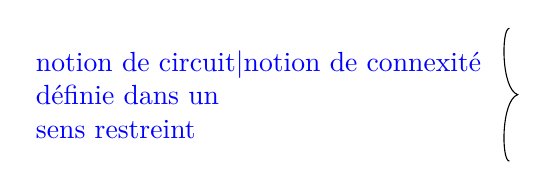
\begin{tikzpicture}
\node[align=left,inner sep=3pt] (m) {\unsure{notion de circuit|notion de connexité}\\\unsure{définie dans un}\\\unsure{sens restreint}};
\draw ([xshift=7pt,yshift=5pt]m.north east)
 .. controls ([xshift=4pt,yshift=5pt]m.north east) and ([xshift=4pt,yshift=2pt]m.east) .. ([xshift=10pt]m.east)
 .. controls ([xshift=4pt,yshift=-2pt]m.east) and ([xshift=4pt,yshift=-5pt]m.south east) .. ([xshift=7pt,yshift=-5pt]m.south east);
\end{tikzpicture}}}
On suppose dorénavant que $\rho$ est \deleted{\unsure{défini}} \inserted{\unsure{prolongé}} sur \unsure{tt} $A$
et que \unsure{$=$} pour l'orientation \unsure{inverse} (ce sont des
propriétés \unsure{combinatoires} de $(A,\sigma,A',\rho)$).
Alors $\rho$ sur $A$ est un \uline{\unsure{autom.}}. Soit $\unsure{\overline S}=A/\rho\supset S$,
$\widehat S\unsure{\subset|=}\overline S$ la partie de $\overline S$ correspondant aux orbites finies.
On peut \unsure{compactifier} \unsure{partiellement} $X$ en \inserted{$\widehat X$}\deleted{\unsure{$\overline X$}}
\unsure{ajoutant} les pts de $\widehat S-S$ (ainsi
que : $\unsure{K^\circ}$\inserted{\unsure{$\simeq\Pi_{0,3}$}}), l'image inverse \inserted{$\widehat A'$} de
$\widehat S$ dans $A$ \inserted{\unsure{contient $A'$ et}}
est \unsure{st.} \unsure{$\forall$} par $\rho$ et $\sigma$
mais \deleted{\unsure{n'est pas|ce n'est pas} néc. égal \unsure{à|avec} $A'$.}
\inserted{: $A$ \unsure{tt entier|est entier}.}

\margin{\figure{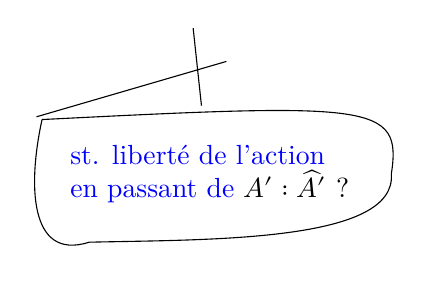
\begin{tikzpicture}
\node[align=left,inner sep=5pt] (m) {\unsure{st. liberté de l'action}\\\unsure{en passant de} $A':\widehat A'$ ?};
\draw ([xshift=-5pt,yshift=4pt]m.north west)
 .. controls ([xshift=-10pt,yshift=-3pt]m.west) and ([xshift=-10pt,yshift=-16pt]m.south west) .. ([xshift=12pt,yshift=-9pt]m.south west)
 .. controls ([yshift=-8pt]m.south) and ([xshift=12pt,yshift=-9pt]m.south east) .. ([xshift=10pt]m.east)
 .. controls ([xshift=14pt,yshift=10pt]m.north east) and ([xshift=3pt,yshift=10pt]m.north east) .. ([xshift=-5pt,yshift=4pt]m.north west);
\draw ([xshift=-7pt,yshift=5pt]m.north west) -- ([xshift=6pt,yshift=25pt]m.north);
\draw ([xshift=-3pt,yshift=9pt]m.north) -- ([xshift=-6pt,yshift=37pt]m.north);
\end{tikzpicture}}}

Les quadruples $(A,\sigma,A',\rho)$ \unsure{satisfaisant} aux
axiomes, \unsure{doivent} \inserted{et tels que $A'=\widehat A'$}
\unsure{s'identifier|s'identifient} aux \deleted{\unsure{triples}} triples
$(A,\sigma,\rho)$ d'un ens. \uline{\unsure{quelc.}} avec un autom.
$\sigma$ d'ordre $2$ \uline{ss pt fixe}, et un autom. $\rho$
\uline{quelc.}. On \unsure{retrouve} $A'$ comme l'ens des
él. de $A$ d'orbite finie sous $\rho$ --- mais on
suppose que $A'\cup\sigma A'=A$.
}

\scanpage{33}
\diagram{\begin{tikzcd}[ampersand replacement=\&,column sep=large,row sep=large]
 0\arrow[r] \& \overset{\omega}{\mathbb Z}\arrow[r,"p"]\arrow[d,"q"'] \& \overset{\widetilde\Pi_0}{\overset{\Vert}{\mathbb Z}}\arrow[r,"\alpha\varphi_p",very thick]\arrow[d] \& \overset{\Pi_0}{\overset{\Vert}{\mathbb Z/p\mathbb Z}}\arrow[r]\arrow[d,equal] \& 0\\
 0\arrow[r,no head,"\overline\omega"'] \& \mathbb Z\arrow[r] \& \widetilde\Pi_0(q)\arrow[r]\arrow[d,"{\substack{\text{\unsure{nul sur }}\widetilde\Pi_0,\\\text{\unsure{can sur }}\mathbb Z\overline\omega}}"] \& \mathbb Z/p\mathbb Z\arrow[r,no head] \& 0\\
 \&\& \mathbb Z/q\mathbb Z \&\&
\end{tikzcd}}
\margin{$\varphi_p:\mathbb Z\longrightarrow\mathbb Z/p\mathbb Z$ hom. can.\\
$\alpha\in(\mathbb Z/p\mathbb Z)^*$\\
\deleted{$\unsure{\beta}\in(\mathbb Z/q\mathbb Z)^*$}}

\diagram{\begin{tikzcd}[ampersand replacement=\&,column sep=large,row sep=large]
 \&\& \overset{\omega}{\mathbb Z}\arrow[r]\arrow[dl,equal] \& \widetilde\Pi_0\arrow[r]\arrow[dl] \& (\mathbb Z/p\mathbb Z\times0)\arrow[dl]\\
 0\arrow[r,no head] \& \overset{\omega}{\mathbb Z}\arrow[r]\arrow[dr,shift right=.6ex] \& \widetilde\Pi_0(q)\arrow[r] \& \mathbb Z/p\mathbb Z\times\mathbb Z/q\mathbb Z\arrow[r,no head] \& 0\\
 \&\& \underset{\omega}{\mathbb Z}\arrow[ul,"q"'{pos=.55},shift right=.6ex]\arrow[r,"\unsure{q}"] \& \underset{\overline\omega}{\mathbb Z}\arrow[ul]\arrow[r,no head] \& 0\times\mathbb Z/q\mathbb Z\arrow[ul]
\end{tikzcd}}
\margin{$\alpha\eta_p$}

\diagram{\begin{tikzcd}[ampersand replacement=\&,column sep=large,row sep=large]
 0\arrow[r,no head] \& \mathbb Z\arrow[r]\arrow[d,equal] \& \widetilde\Pi_0(q)\arrow[r,no head] \& \mathbb Z/p\mathbb Z\times\mathbb Z/q\mathbb Z\arrow[r,no head] \& 0\\
 0\arrow[r,no head] \& \mathbb Z\arrow[r,no head] \& \widetilde\Pi'_0\arrow[r]\arrow[u] \& \mathbb Z/\mu\mathbb Z\arrow[r,no head]\arrow[u,"\delta",very thick] \& 0
\end{tikzcd}}

\deleted{\unsure{L'extension est} \illegible{1} :}
\[
 \unsure{\zeta'|\xi'}\deleted{\unsure{\zeta|\xi}}=
 \mathrm{cl}(\widetilde\Pi'_0)\in
 \operatorname{Ext}^{\unsure{1}}_{\deleted{\unsure{\mathbb Z}}}
 (\mathbb Z/\mu\mathbb Z,\mathbb Z)\simeq\mathbb Z/\mu\mathbb Z
\]
\[
 \deleted{\unsure{=}}\quad
 \unsure{\zeta'|\xi'}=
 \delta^*\!\left(
 \underbrace{\mathrm{cl}(\widetilde\Pi_0\unsure{(q)|q})}_{\unsure{\zeta|\xi}\,\in\,\operatorname{Ext}^1(\mathbb Z/p\mathbb Z\times\mathbb Z/q\mathbb Z,\mathbb Z)}
 \right)\unsure{'}
\]
\[
 \unsure{\zeta|\xi}=
 \mathrm{pr}_1^*\!\left(\underbrace{\mathrm{cl}(\widetilde\Pi_0)}_{\alpha\eta_p}\right)
 +\mathrm{pr}_2^*\!\left(\underbrace{\mathrm{cl}(\mathbb Z)}_{\eta_q}\right)
\]
\[
\begin{array}{ll}
 \delta_p:\mathbb Z/\mu\mathbb Z\mathrel{\overset{\mathrm{can}}{-}}\mathbb Z/p\mathbb Z
 &\unsure{\zeta'|\xi'}=\deleted{q'\eta_\mu+p'\eta_\mu}\\[1ex]
 \delta_q:\mathbb Z/\mu\mathbb Z\mathrel{\overset{\mathrm{can}}{-}}\mathbb Z/q\mathbb Z&\\[1ex]
 \delta_p^*(\eta_p)=q'\eta_\mu & \delta_p^{\unsure{*|' }}(\alpha\eta_p)=q'\alpha\eta_\mu\\[1ex]
 \delta_q^{\unsure{*|'}}(\eta_q)=p'\eta_\mu &
\end{array}
\]
\margin{32}

\scanpage{34}
\deleted{$\unsure{4)}\ \unsure{\widetilde{\mathrm{Sl}}}(2,\mathbb Z)\simeq
\unsure{\mathcal T_{1,1}}\,\unsure{\mathrm{SL}}\,\unsure{\Pi}$}

1)
\[
\begin{gathered}
 S\mathcal T_{11}\simeq\widetilde{\mathrm{Sl}}(2,\mathbb Z)
 \simeq\{\rho,\sigma\mid\underbrace{\rho^3=\sigma^2}_{\omega}\}
 \simeq
 \underset{\substack{\Vert\\\{\rho,\sigma\mid\rho^3=\sigma^2=1\}}}{\Pi_{0,3}^D}
 \times_{\unsure{\mathbb Z/6\mathbb Z}}\mathbb Z\\
 \simeq S\Pi_{0,3}^D
\end{gathered}
\]
\inserted{\deleted{$\unsure{\alpha}$}
\diagram{\begin{tikzcd}[ampersand replacement=\&,row sep=small]
 \rho\arrow[r,mapsto]\&2\\
 \sigma\arrow[r]\&3
\end{tikzcd}}}

% Le bloc suivant est écrit tête-bêche par rapport à la ligne précédente.
\diagram{\begin{tikzcd}[ampersand replacement=\&,column sep=large,row sep=large]
 \widetilde\Pi\arrow[r,no head]\arrow[dd,no head]\&\unsure{\Pi}\arrow[r,no head]\arrow[d]\&\Pi'\arrow[r]\arrow[dd,Rightarrow]\&\Pi\arrow[dd]\\
 \&\mathbb D_3''\arrow[dd]\&\&\\
 \mathbb Z\arrow[rr]\&\&\mathbb Z/12\mathbb Z\arrow[r]\arrow[d]\&\mathbb Z/6\mathbb Z\arrow[d]\\
 \&\unsure{\mathbb Z/}\&\mathbb Z/4\mathbb Z\arrow[r]\&\mathbb Z/2\mathbb Z
\end{tikzcd}}
\margin{$\Pi_0=\mathbb Z/6\mathbb Z$}
\margin{$\Pi_0\times\unsure{7|1}$}
\diagram{\begin{tikzcd}[ampersand replacement=\&,column sep=large,row sep=large]
 \mathbb Z\arrow[r,no head]\&\widetilde\Pi(4)\arrow[r]\&\Pi\times\mathbb Z/4\mathbb Z\arrow[r,no head]\arrow[d]\&1\\
 \&\widetilde\Pi\arrow[u,"?"']\arrow[r,"\uline{\unsure{cart}}"]\&\Pi'\&
\end{tikzcd}}

% Billet préexistant, à lire après une rotation de 90 degrés.
\margin{27-11-81}
M. Grothendieck

A remplir d'urgence

Merci

\uline{R. \unsure{Boucher}}
\margin{33}

\scanpage{35}
\[
 (p'+q'\alpha)\eta_\mu
\]
\[
 p=6,\ q=4\qquad(\alpha=-1\ ?)
\]
\[
 \deleted{\unsure{p}}\ \mu=12\qquad p'=3,\ q'=2
\]
\[
 \deleted{\unsure{p'+}}\ (3-2)\eta_\mu\ !
\]
\figure{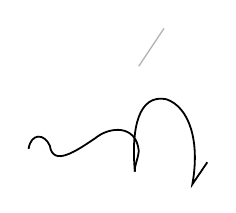
\begin{tikzpicture}[x=1cm,y=1cm]
 \draw[line width=.5pt,opacity=.3] (1.4,1.7)--(1.72,2.18);
 \draw[line width=.65pt] (0,.65) .. controls (.03,.85) and (.2,.85) .. (.27,.69)
 .. controls (.31,.42) and (.6,.62) .. (.84,.78)
 .. controls (1.03,.94) and (1.37,.96) .. (1.4,.62)
 .. controls (1.38,.48) and (1.34,.43) .. (1.35,.36);
 \draw[line width=.65pt] (1.35,.36) .. controls (1.3,.92) and (1.4,1.35) .. (1.75,1.28)
 .. controls (2.04,1.18) and (2.18,.75) .. (2.08,.2)
 --(2.27,.48);
\end{tikzpicture}}

$\cdot$
\diagram{\begin{tikzcd}[ampersand replacement=\&,column sep=large,row sep=small]
 \Pi_{0,3}^D\arrow[r,"{-\alpha}"{draw,circle,inner sep=1pt},very thick]\&\mathbb Z/6\mathbb Z\\
 \rho\arrow[r,mapsto]\&-2\ \mathrm{mod}\ 6\\
 \sigma\arrow[r,mapsto]\&3\ \mathrm{mod}\ 6\\[1ex]
 \varepsilon_0=\sigma\rho\arrow[r,mapsto,very thick]\&1\ \mathrm{mod}\ 6\\
 \rho_0=\varepsilon_0^2\arrow[r,mapsto]\&2\ \mathrm{mod}\ 6
\end{tikzcd}}
\deleted{$\unsure{\varphi}$}
% Marques très pâles à droite des résidus; possible transparence du verso.
\margin{$\unsure{\Gamma|\sqrt{\phantom{x}}}$\\$\unsure{\xi_0\prime|\xi_0}$\\$\unsure{t\prime r|t\prime h}$}

\margin{défini directement par l'action de $\Pi_{0,3}^D$ sur le
\unsure{revêt}\deleted{\unsure{ement}} principal de $(U_{0,3},\mathfrak S_3)$
de groupe $\mathbb Z/6\mathbb Z$, défini par
la \unsure{multisection|multiplication} \inserted{canonique} de
\deleted{$\unsure{\mathcal O(1)}$}$\mathcal O_{U_{0,3}}(1)^*$
$=PU_{0,3}$}

\[
 \widetilde\Pi_{0,3}^D
\]
\deleted{$\mathcal O\unsure{(1)}$}
\diagram{\begin{tikzcd}[ampersand replacement=\&,column sep=small,row sep=large]
 U'_{0,3}\arrow[rr,phantom,"\subset"]\arrow[dr,no head,"{\mu_6\text{-}\unsure{\mathrm{rev}^{\mathrm t}}}"']\&\&PU_{0,3}\arrow[dl,no head]\&\unsure{+}\\
 \&U_{0,3}\&\&
\end{tikzcd}}
\deleted{$\unsure{\longrightarrow}$}

\diagram{\begin{tikzcd}[ampersand replacement=\&,column sep=large,row sep=large]
 \&\Pi_{0,3}^D\arrow[r,"{\alpha'}"{draw,circle,inner sep=1pt},very thick]\&\mathbb Z/6\mathbb Z\\
 \pi_1(PU_{0,3},\mathfrak S_3)\arrow[r,equal]\&\widetilde\Pi_{0,3}^D\arrow[u]\arrow[r]\&\mathbb Z\arrow[u]\\
 \&\omega'\in\mathbb Z\arrow[u]\arrow[r,"\unsure{=}"]\&\mathbb Z\arrow[u,"6"]
\end{tikzcd}}

\diagram{\begin{tikzcd}[ampersand replacement=\&,column sep=large,row sep=large]
 1\arrow[r]\&\mathbb Z\arrow[r]\arrow[d,equal]\&
 \underset{\substack{\Vert\\\pi_1(PU_{0,3},\mathfrak S_3\times\mu_4)}}{\widetilde\Pi_{0,3}^D(4)}\arrow[r,very thick]\&
 \Pi_{0,3}^D\times\mathbb Z/4\mathbb Z\arrow[r]\&1\\
 1\arrow[r,no head]\&\mathbb Z\arrow[r]\&\widetilde{\mathcal T}_{11}\arrow[u,bend left=20]\arrow[r,Rightarrow]\&
 \mathcal T_{1,1}=\Pi_{0,3}^D\times_{\mathbb Z/2\mathbb Z}\mathbb Z/4\mathbb Z\arrow[u,hook]\&
\end{tikzcd}}

\deleted{$\unsure{\widetilde\Pi_{0,3}^D}\,\unsure{\mathbb Z/4\mathbb Z}\longrightarrow$}
\[
\begin{array}{ll}
 \widetilde\Pi_{0,3}^D\ni\widetilde\rho^{\unsure{\sharp|'}}=(\rho,-2)
 &\widetilde\rho^{\unsure{\sharp}3}=\widetilde\sigma^{\unsure{\sharp}2}=\omega'\\
 \hfill\widetilde\sigma^{\unsure{\sharp|'}}=(\sigma,-3)&
\end{array}
\]
\diagram{\begin{tikzcd}[ampersand replacement=\&,column sep=small,row sep=small]
 \widetilde\rho,\arrow[d]\&\widetilde\sigma\arrow[d]\&
 \in\widetilde\Pi_{0,3}^D=
 \left\{\widetilde\rho,\widetilde\sigma\mid
 \underbrace{\widetilde\rho^3=\widetilde\sigma^2}_{\unsure{\omega'^{-1}|\widetilde\omega^{-1}}=\unsure{\omega|\infty}}
 \deleted{\unsure{\omega\in\mathbb Z}}\right\}\\
 \rho\&\sigma\&\simeq\widetilde{\mathcal T}_{11}
\end{tikzcd}}
\margin{34}

\scanpage{36}
\diagram{\begin{tikzcd}[ampersand replacement=\&,column sep=large,row sep=large]
 \&\&\left\{\rho,\sigma\mid\underbrace{\rho^3=\sigma^2}_{\omega'^{-1}=\omega}\right\}\deleted{\unsure{\omega|\infty}}\arrow[d,equal]\&\&\\
 1\arrow[r,no head]\&\overset{\omega'=\unsure{\omega^{-1}|\overline\omega'}}{\mathbb Z}\arrow[r]\arrow[d,equal]\&S\Pi_{0,3}^D\arrow[r]\arrow[d]\&\Pi_{0,3}^D\arrow[r,no head]\arrow[d]\&1\\
 1\arrow[r,no head]\&\mathbb Z\arrow[r]\&S\Pi_{0,3}^D(4)\arrow[r]\&\Pi_{0,3}^D\times\mathbb Z/4\mathbb Z\arrow[r,no head]\&1\\[4em]
 1\arrow[r]\&\underset{\omega^2}{\mathbb Z}\arrow[r]\arrow[u,very thick]\&S\mathcal T_{11}\arrow[r]\arrow[u,very thick,"{\underbrace{\begin{gathered}\rho\mapsto\rho\overline\omega^2\\\sigma\mapsto\sigma\overline\omega^3\\\omega\longrightarrow\overline\omega^2\\\omega^2\longrightarrow\overline\omega^4=\omega'\end{gathered}}}"]\&\mathcal T_{11}\arrow[u,hook,"{\substack{\rho\mapsto(\rho,2)\\\sigma\mapsto(\sigma,3)}}"]\&\omega\longrightarrow(1,2)
\end{tikzcd}}
\margin{$S\Pi_{0,3}^D(4)=\left\{\rho,\sigma,\overline\omega\mid\begin{gathered}\rho^3=\sigma^2=\overline\omega^{-4}\\\overline\omega\ \text{central}\end{gathered}\right\}$\\
NB $\unsure{\dot{\overline\omega}|\overline\omega}^{4}=\unsure{\omega^{-1}}$\\
$=\omega'\deleted{\unsure{\omega}}$}

% Groupe et flèche au pied du feuillet, écrits tête-bêche.
\diagram{\begin{tikzcd}[ampersand replacement=\&,column sep=large]
 \overbrace{S\Pi_{0,3}^D(4)}^{\pi_1(U_{0,3},\mathfrak S_3\times\mu_4)}\arrow[r]\&\Pi_{0,3}^D
\end{tikzcd}}
\margin{35}

\scanpage{37}
% not manuscript: formulaire vierge « ANNEXE II », renseignements à fournir par le candidat devant soutenir une thèse de doctorat d'État, Université des Sciences et Techniques du Languedoc, imprimé tête-bêche.
\margin{36}

\end{document}
